\documentclass[]{article}
\usepackage[utf8]{inputenc}
\usepackage{graphicx, float, url, hyperref, lscape, afterpage, amsthm, amsmath, amsfonts, booktabs, amssymb, subfig, mhchem}
\usepackage[margin=2in]{geometry}

\title{CS297 Problem Set 1}
\author{B Beltran, D Hostallero, F Rayo}
\date{\today}

\begin{document}
	
	\maketitle
	
	\section*{Chapter 2}
	\subsection*{2.1}
	Given $\dot{x} = \sin x$ as a flow on a line.
	\\
	
	\textbf{2.1.1} The fixed points are when $\sin x = 0$, that is, $x=n\pi,$ $\forall$ $n$ $\in \mathbb{N}.$
	\\
	
	\textbf{2.1.2} The flow has greatest velocity to the right when $\sin x = 1$, its maximum positive value. Thus, $x = \frac{\pi}{2} + 2n\pi,$ $\forall$ $n$ $\in \mathbb{N}.$
	\\
	
	\textbf{2.1.3. A.} The flow's acceleration is given by $\ddot{x}=\frac{d}{dt}(\dot{x})$.
	\begin{align*}
	\ddot{x}&=\frac{d}{dt}(\dot{x})\\
	&=\frac{d}{dt}(\sin x)\\
	&=\dot{x}\cos x\\
	&=\sin x \cos x\\
	\ddot{x}&=\frac{1}{2}\sin 2x
	\end{align*}
	\\
	
	\textbf{2.1.3 B.} The flow has maximum positive acceleration when $\ddot{x}=\frac{1}{2}\sin 2x$ is at its maximum positive value. This occurs when $\sin 2x = 1$.
	\begin{align*}
	\sin 2x &= 1\\
	2x &= \frac{\pi}{2} + 2n\pi ,\forall n \in \mathbb{N}\\
	x &= \frac{\pi}{4} + n\pi, \forall n \in \mathbb{N}
	\end{align*}
	\\
	
	\textbf{2.1.5} An example of a mechanical system that is approximately governed by $\ddot{x} = \sin x$ is an overdamped pendulum, where $x$ is the angle between the pendulum and the upward vertical. At $x^* = 0$, the pendulum is balanced above the pivot, which makes it a fixed point due to lack of movement. This is unstable since a slight push will make the pendulum oscillate, and eventually rest at $x^* = \pi$, the downward vertical. At $x^* = \pi$, the downward vertical, the pendulum is at rest so it is a fixed point. A slight push will make the pendulum oscillate, but eventually come to rest in the same position. Thus is is intuitively stable.
	
	\subsection*{2.2}
	
	\subsection*{2.2.2} 
	$\dot x = 1 - x^{14}$\\
	The fixed points at -1 is an unstable fixed point, while the fixed point at 1 is a stable fixed point.
	\begin{figure}[H]
		\centering
		\subfloat[graph of $\dot x$]
		{{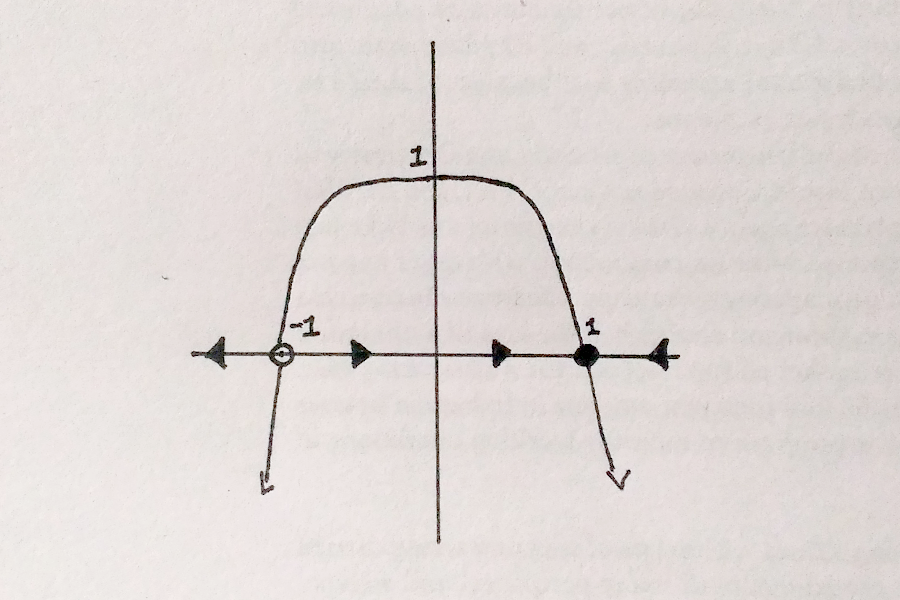
\includegraphics[width=5cm]{img/2-2-2a.png} }}%
		\qquad
		\subfloat[x(t) for different initial conditions]
		{{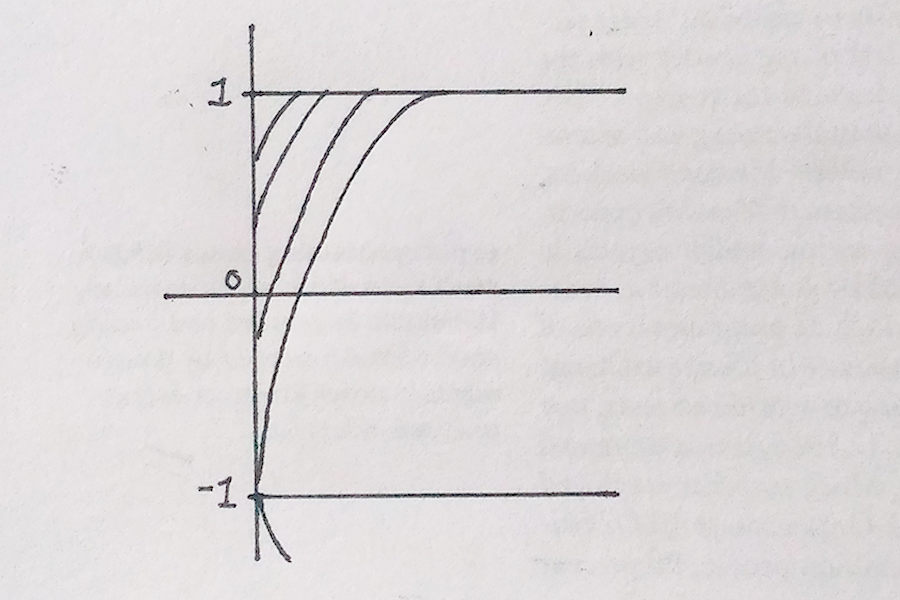
\includegraphics[width=5cm]{img/2-2-2b.png} }}%
		\caption*{}%
		\label{fig:example}%
	\end{figure}
	
	\subsection*{2.2.4} $\dot x = e^x sin(x)$\\
	The fixed points are at $2k\pi$ for integer k. The fixed point is stable if k is odd, and unstable if k is even.
	
	\begin{figure}[H]
		\centering
		\subfloat[graph of $\dot x$]
		{{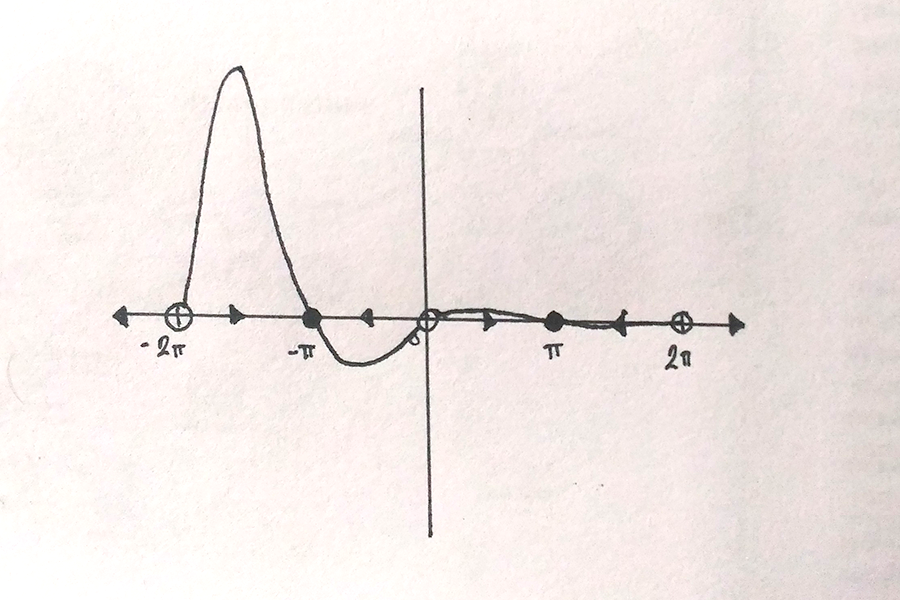
\includegraphics[width=5cm]{img/2-2-4a.png} }}%
		\qquad
		\subfloat[x(t) for different initial conditions]
		{{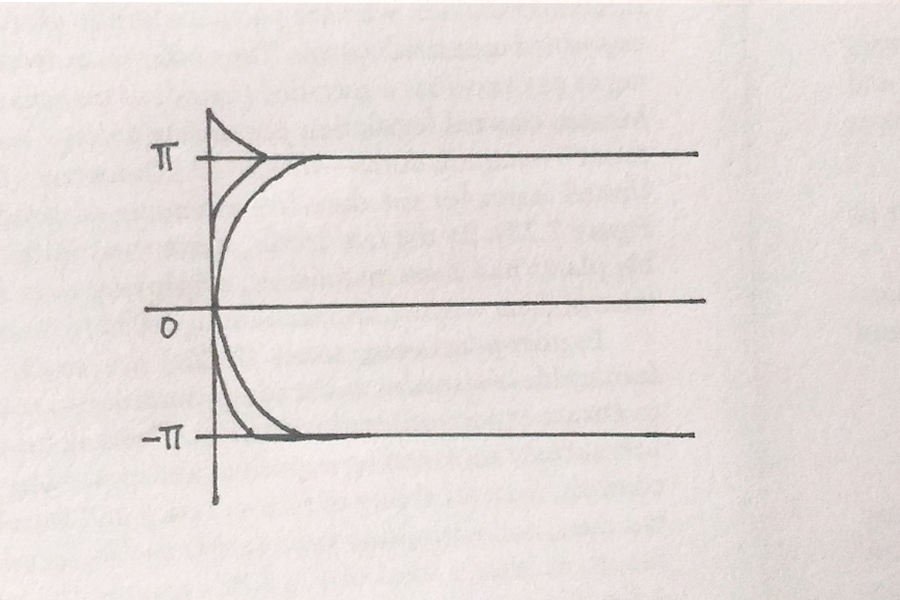
\includegraphics[width=5cm]{img/2-2-4b.png} }}%
		\caption*{}%
		\label{fig:example}%
	\end{figure}
	
	\subsection*{2.2.5} $\dot x = 1 - 2cos(x)$\\
	There unstable fixed points at $2k\pi + \frac{\pi}{3}$, and stable fixed points at $2k\pi - \frac{\pi}{3}$, where k is an integer
	\begin{figure}[H]
		\centering
		\subfloat[graph of $\dot x$]
		{{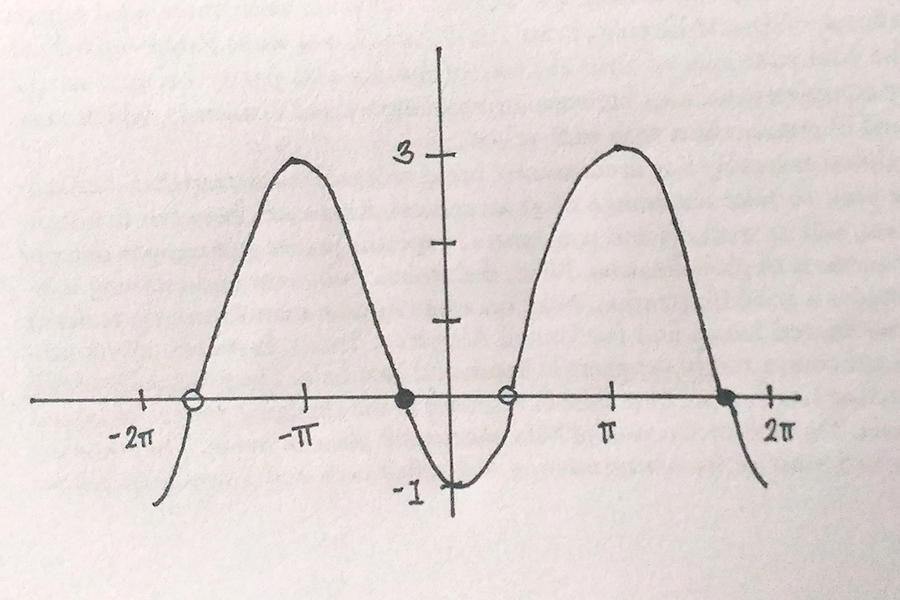
\includegraphics[width=5cm]{img/2-2-6a.png} }}%
		\qquad
		\subfloat[x(t) for different initial conditions]
		{{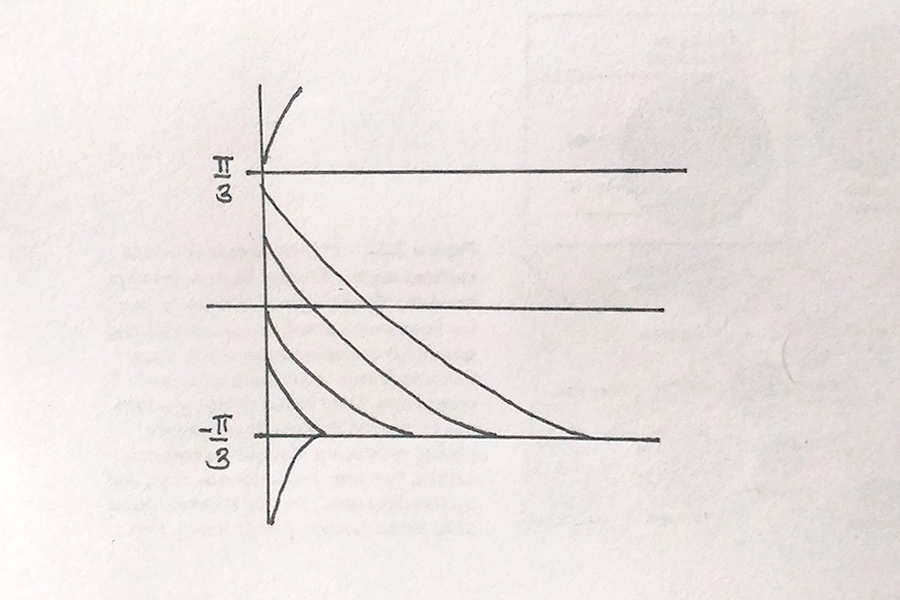
\includegraphics[width=5cm]{img/2-2-6b.png} }}%
		\caption*{}%
		\label{fig:example}%
	\end{figure}
	
	\subsection*{2.2.13 A} The analytical solution to $m \dot v = mg - kv^2$ is given by the following:
	\begin{align*}
	m \dot v & = mg - kv^2 \\
	\int \frac{m}{mg-kv^2} dv & = \int t dt\\
	-\frac{m}{k} \int \frac{dv}{v^2 - mg/k} & = t + C
	\end{align*}
	
	let $a = \sqrt{\frac{mg}{k}}$
	
	\begin{align*}
	-\frac{m}{k} \int \frac{1}{v^2 - a^2} dv & = t + C\\
	-\frac{m}{k} \frac{1}{2a} ln \Bigg(\frac{v - a}{v +  a}\Bigg) & = t + C\\
	\frac{v-a}{v+a} & = e^{-2t\sqrt{\frac{gk}{m}}} e^{-2C\sqrt{\frac{gk}{m}}}
	\end{align*}
	
	let $C_1 = e^{-2C\sqrt{\frac{gk}{m}}}$
	
	\begin{align*}
	\frac{v-a}{v+a} & = e^{-2t\sqrt{\frac{gk}{m}}} C_1\\
	v-a & = e^{-2t\sqrt{\frac{gk}{m}}} C_1 (v + a)\\
	v & = \sqrt{\frac{mg}{k}} \Bigg(\frac{1 + e^{-2t\sqrt{\frac{gk}{m}}}C_1}{1 - e^{-2t\sqrt{\frac{gk}{m}}}C_1}\Bigg)\\
	\end{align*}
	
	Assuming that $v(0) = 0$, then $C_1 = -1$
	
	\begin{align*}
	v(t) & = \sqrt{\frac{mg}{k}} (\frac{1 - e^{-2t\sqrt{\frac{gk}{m}}}}{1 + e^{-2t\sqrt{\frac{gk}{m}}}})\\
	& = \sqrt{\frac{mg}{k}} tanh \Bigg(\sqrt{\frac{gk}{m}} t\Bigg)
	\end{align*}
	
	\subsection*{2.2.13. B.} As $t \rightarrow \infty$, $v(t) \rightarrow \sqrt{\frac{mg}{k}}$
	
	\subsection*{2.2.13. C.} The fixed point at $t = \sqrt{\frac{mg}{k}}$ is a stable fixed point as shown in the plot. Therefore, the formula for the terminal velocity can be rederived as $v_{t} = \sqrt{\frac{mg}{k}}$\\
	
	\begin{figure}[H]
		\centering
		\subfloat[graph of v(t)]
		{{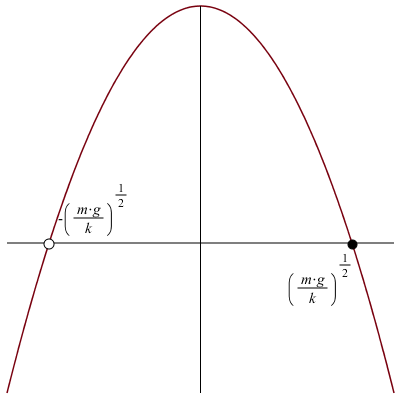
\includegraphics[width=5cm]{img/2-2-13c.png} }}%
		\qquad
		\subfloat[slope field of v(t)]
		{{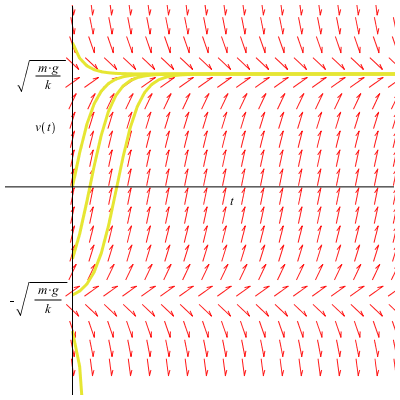
\includegraphics[width=5cm]{img/2-2-13c2.png} }}%
		\caption*{}%
		\label{fig:example}%
	\end{figure}
	
	\subsection*{2.2.13. D}
	
	\begin{align*}
	V_{avg} & = \frac{31400-2100}{116}\\
	& = 252.59 ft/sec
	\end{align*}
	
	\subsection*{2.2.13. E}
	\begin{align*}
	\dot s & = v \\
	\frac{ds}{dt} & =  \sqrt{\frac{mg}{k}} tanh(\sqrt{\frac{gk}{m}} t) \\
	\int ds & = \int \sqrt{\frac{mg}{k}} \frac{sinh(\sqrt{\frac{gk}{m}} t)}{cosh(\sqrt{\frac{gk}{m}} t)} dt \\
	s + C & = \int \sqrt{\frac{mg}{k}} \frac{e^{\sqrt{\frac{gk}{m}} t} - e^{-\sqrt{\frac{gk}{m}} t}}{e^{\sqrt{\frac{gk}{m}} t} + e^{-\sqrt{\frac{gk}{m}} t}} 
	\end{align*}
	
	let $u = e^{\sqrt{\frac{gk}{m}} t} + e^{-\sqrt{\frac{gk}{m}} t}$ \\
	$du = \sqrt{\frac{gk}{m}} (e^{\sqrt{\frac{gk}{m}} t} - e^{-\sqrt{\frac{gk}{m}} t}$
	
	\begin{align*}
	s + C & = \frac{m}{k} \int \frac{du}{u} \\
	& = \frac{m}{k} ln (cosh(\sqrt{\frac{gk}{m}} t))\\
	& = \frac{V^2}{g} ln (cosh(\frac{gt}{V}))
	\end{align*}
	
	Since $s(0) = 0$, then
	\begin{equation*}
	s(t) = \frac{V^2}{g} ln (cosh(\frac{gt}{V}))   
	\end{equation*}
	
	We then graph $s = 29300$ and $s = \frac{V^2}{g} ln \Big(cosh\Big(\frac{gt}{V}\Big)\Big)$ and find their intersection. The intersection is at about $v = 265.68$ as seen in the zoomed-in graph below.
	
	\begin{figure}[H]
		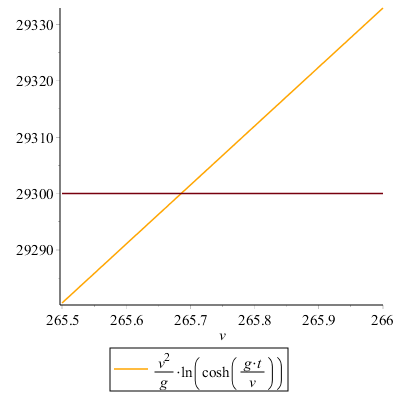
\includegraphics[width=\textwidth]{img/2-2-13e.png}
	\end{figure}
	
	We then use $v = 265.68$ to find the drag constant $k$. Note that the weight in pounds is already $mg$.
	\begin{align*}
	v_{t} &= \sqrt{\frac{mg}{k}}\\
	k &= \frac{mg}{v_t^2}\\
	&= \frac{261.2}{265.68^2}\\
	k &= 3.70 \times 10^{-3}
	\end{align*}
	
	\subsection*{2.3.2}
	\textbf{A.} Given $\dot{x} = k_1ax-k_2x^2$, the fixed points are
	\begin{align*}
	0 &= k_1ax-k_2x^2\\
	0 &= x(k_1a-k_2x)\\
	x &= 0, \quad x = \frac{k_1}{k_2}a
	\end{align*}
	To check for stability, we can substitute the fixed points at the second derivative. If $\ddot{x} > 0$, it is unstable; otherwise it is stable.
	\begin{align*}
	\ddot{x}|_{x=0} &= k_1a\\
	\ddot{x}|_{x=\frac{k_1a}{k_2}} &= -k_1a
	\end{align*}
	Since $k_1$, $a$ and $k_2$ are both positive, the fixed point at $x=0$ is unstable and $x=\frac{k_1a}{k_2}$ is stable.\\
	\textbf{B.} Using different initial values, the graph of $x(t)$ is given below.
	
	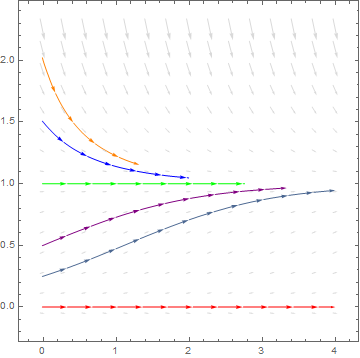
\includegraphics[width=\textwidth]{232a.png}
	
	Note that the fixed points and the asymptotic limit still holds.
	
	\subsection*{2.3.4}
	\textbf{A.} We need to find $N$ that gives the maximum growth rate $\dot{N}/N$. It is given by
	
	\begin{align*}
	\frac{\dot{N}}{N} &= r-a(N-b)^2\\
	0&=-2a(N-b) \to N=b
	\end{align*}
	It is indeed the maximum point since it has negative second derivative with a parabola facing downward. The roots of $\frac{\dot{N}}{N}$ which can be solved by
	\begin{align*}
	0 &= r-a(N-b)^2\\
	N &= b \pm \sqrt{\frac{r}{a}}
	\end{align*}
	
	Next, $N=b$ should be between these two roots that can be expressed mathematically as
	\begin{align*}
	\left(\sqrt{\frac{r}{a}}+b\right) - \left(-\sqrt{\frac{r}{a}}+b\right) &= b\\
	2\sqrt{\frac{r}{a}}=b \to
	4\frac{r}{a}&=b^2
	\end{align*}
	Which requires that $a>0$, $r>0$ and $b \in \mathbb{R}$ to achieve the Allee effect.
	\\
	
	\textbf{B.} To get the fixed points we need to set $\dot{N}=0$:
	\begin{align*}
	0 &= N(r-a(N-b)^2)\\
	N_1 &= 0, \quad N_{2,3} = b \pm \sqrt{\frac{r}{a}}
	\end{align*}
	
	To classify the stability, evaluate the fixed points on its second derivative.
	\begin{align*}
	\ddot{N} &= 2+4N-3N^2\\
	\ddot{N}|_{N=N_1} &= 3,\quad \text{unstable}\\
	\ddot{N}|_{N=N_2} &= 2 \left(\sqrt{3}-3\right),\quad \text{stable}\\
	\ddot{N}|_{N=N_2} &= -2 \left(3+\sqrt{3}\right), \quad \text{stable}
	\end{align*}
	
	\textbf{C.} Using $a=1,r=1$ and $b=2$, the solution with different initial conditions are given below:
	
	\textbf{D.} The graph below compares $N(t)$ versus the logistic equation with $k=3$ using the same set of initial values.
	
	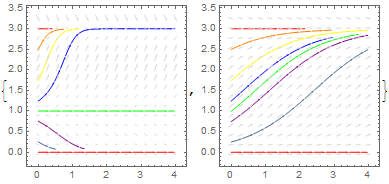
\includegraphics[width=\textwidth]{234b.png}
	
	The main difference is that Allee effect allows an unstable point between $N=0$ and $N=k$. This can be viewed as the optimum population that will not grow or will not die. Slightly adding or subtracting from the population makes the system grow into max capacity or die. On the other hand the logistic equation has only two fixed points $N=0$ and $N=k$. Any intermediate population allows them to grow to max capacity.
	
	\subsection*{2.4}
	\textbf{2.4.2}
	\begin{align*}
	f(x) &= x(1-x)(2-x) \\
	fixed points:x &= 0, 1, 2 \\
	f(x) &= 2x - 3x^2 + x^3 \\
	f'(x) &= 2-6x + 3x^2
	\end{align*}
	Evaluating f'(x) at the fixed points:
	\begin{align*}
	f'(0) &= 2, unstable \\ 
	f'(1) &= 3 - 6 + 2 = -1 , stable \\ 
	f'(2) &= 12 - 12 + 2 = 2, unstable
	\end{align*}
	\\
	\textbf{2.4.4}
	\begin{align*}
	f(x) &= x^2(6-x) \\
	fixed points:x &= 0, 6 \\
	f(x) &= 6x^2 - x^3\\
	f'(x) &=12x - 3x^2
	\end{align*}
	Evaluating f'(x) at the fixed points:
	\begin{align*}
	f'(0) &= 0, half stable \\ 
	f'(6) &= 72 - 108 = -36, stable 
	\end{align*}
	\\
	\textbf{2.4.6}
	\begin{align*}
	f(x) &= \ln x \\
	fixed points:x &= 1 \\
	f'(x) &= \frac{1}{x}
	\end{align*}
	Evaluating f'(x) at the fixed points:
	\begin{align*}
	f'(1) &= 1, unstable 
	\end{align*}
	\\
	\textbf{2.4.8}
	\begin{align*}
	f(N) &= -aN \ln (bN) \\
	fixed points:N &= \frac{1}{b} \\
	f'(N) &= = -a(1+\ln (bN))
	\end{align*}
	Evaluating f'(N) at the fixed points:
	\begin{align*}
	f'(\frac{1}{b}) &= -a(1+\ln (1)) &= -a\\
	-a &< 0, stable, since a > 0
	\end{align*}
	
	
	\subsection*{2.5}
	\textbf{2.5.2}
	
	\begin{align*}
	\frac{dx}{dt} = 1 + x^2\\
	\int \frac{1}{1  + x^2} dx = \int dt\\
	tan^-1(x) = t + C\\
	\end{align*}
	
	The solution only exists for $-\frac{\pi}{2} < t < \frac{\pi}{2}$ so $x(t) \rightarrow \infty$ as $t \rightarrow \pm\frac{\pi}{2}$\\
	Note that $1 + x^10 > 1 + x^2$ for $x > 1$. This means $1 + x^10$ will also reach infinity at finite time.\\
	
	\subsection*{2.6.1}
	The simple harmonic oscillator $m\ddot{x}=-kx$ oscillates in one direction \textit{physically}, but the oscillation is described by two variables, namely velocity $\dot{x}=v$ and acceleration $\dot{v}=-\frac{k}{m}x$ making it a two-dimensional system, in a theoretical sense.
	
	\subsection*{2.6.2}
	Consider the integrals that should be both true:
	\begin{align*}
	\int_{t}^{t+t} f(x)\frac{dx}{dt}dt &= \int_{x(t)}^{x(t+T)}f(x)dx\\
	\int_{t}^{t+t} f(x)\frac{dx}{dt}dt &= \int_{t}^{t+T}[f(x)]^2dx \geq 0
	\end{align*}
	
	The equalities are achieved using chain rule and the fact that $\dot{x}=f(x)$. However, these equalities satisfy a trivial solution, when $x(t)=x(t+s)=0 $ for all $0<s<t$. Therefore we have derived a contradiction and it is impossible to have oscillations for a one-dimensional system. \qedsymbol
	
	\subsection*{2.7}
	\textbf{2.7.2} Given $\dot{x} = 3$ , there are no fixed points. Then from $-\frac{dv}{dx} = 3$, $V(x) = -3x$.
	%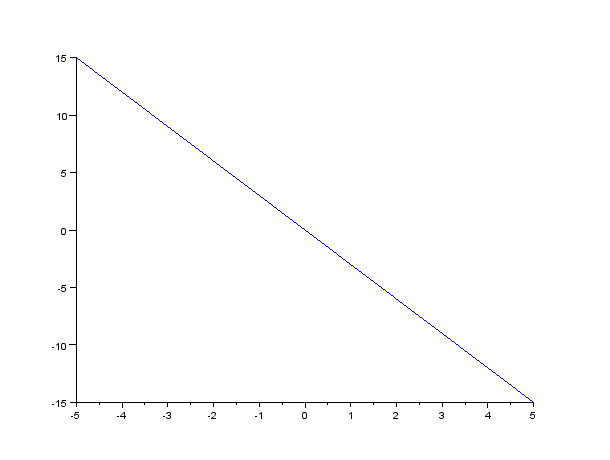
\includegraphics[width=\textwidth]{272.png}
	\\
	
	\textbf{2.7.4} Given $\dot{x} = 2 + \sin x$ , there are no fixed points since $-1 \leq \sin x \leq  1$. That is, $1 \leq \dot{x} \leq 3$. Then from $-\frac{dv}{dx} = 2 + \sin x$, $V(x) = \cos x - 2x$.
	%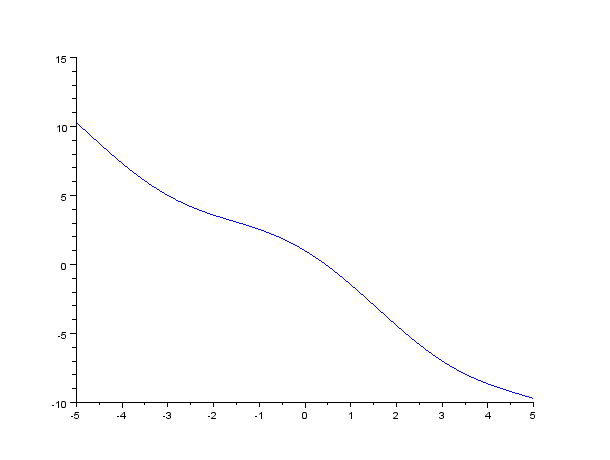
\includegraphics[width=\textwidth]{274.png}
	\\
	
	\textbf{2.7.6} Taking the critical points for $\dot{x} = r + x - x^2$, $\ddot{x} = 1 - 3x^2$ which is $0$ when $x = \pm \frac{1}{\sqrt{3}}$. Substituting these into $\dot{x}$, we get $r = \mp \frac{2}{\sqrt{27}}$. Thus as seen in the plot of the potential, $r < \frac{2}{\sqrt{27}}$ , there are three fixed points. There is one unstable in the center, and two stable fixed points on either side. In the case of $r = 0$, the unstable fixed point is at $x = 0$ and the stable fixed points are at $x = \pm 1$.  On the other hand if $ r \geq \frac{2}{\sqrt{27}}$, there is only one fixed point. \\
	From $-\frac{dv}{dx} = r + x - x^2$, $V(x) = \frac{1}{4}x^4 - \frac{1}{2}x^2 - rx$.
	%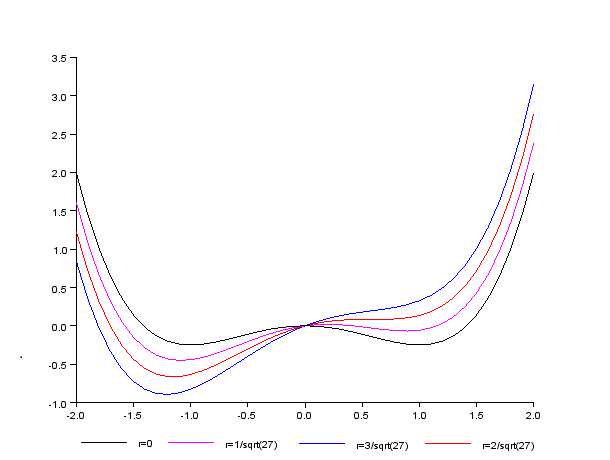
\includegraphics[width=\textwidth]{2761.png}
	
	\subsection*{2.8.2 A} $\dot x = x$
	\begin{figure}[H]
		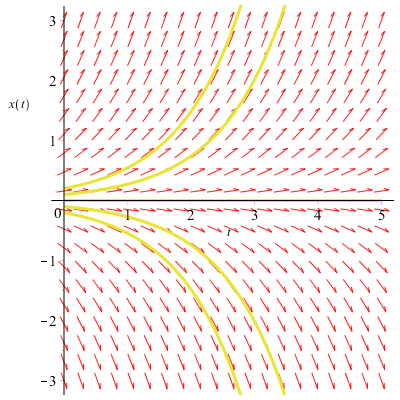
\includegraphics[width=\textwidth]{img/2-8-2a.png}
	\end{figure}
	
	\subsection*{2.8.2 B} $\dot x = 1 - x^2$
	\begin{figure}[H]
		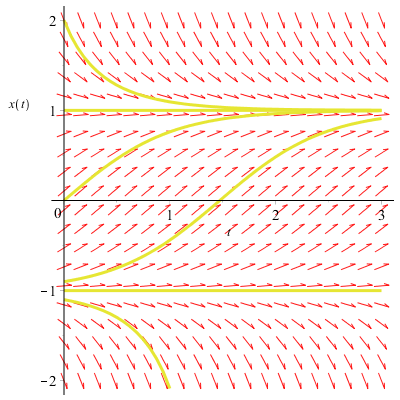
\includegraphics[width=\textwidth]{img/2-8-2b.png}
	\end{figure}
	
	\subsection*{2.8.2 C} $\dot x = 1 - 4x(1-x)$
	\begin{figure}[H]
		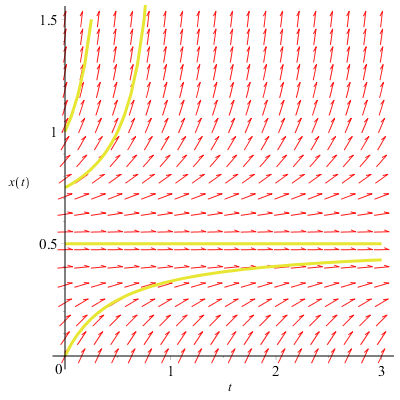
\includegraphics[width=\textwidth]{img/2-8-2c.png}
	\end{figure}
	
	\subsection*{2.8.2 D} $\dot x = sin(x)$
	\\
	\begin{figure}[H]
		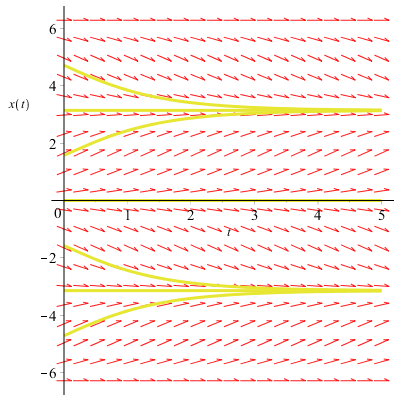
\includegraphics[width=\textwidth]{img/2-8-2d.png}
	\end{figure}
	
	\subsection*{2.8.4 A}
	\begin{align*}
	\frac{dx}{dt} &= -x\\
	\int \frac{dx}{-x} &= \int dt\\
	x &= e^{-(t + c)}\\
	\end{align*}
	
	If $x(0) = 1$, then $C = 0$\\
	
	\begin{align*}
	x(t) &= e^{-t}\\
	x(1) &= e^{-1}\\
	&= 0.3679
	\end{align*}
	
	
	\subsection*{2.8.4 B}
	\begin{align*}
	&\Delta t = 1: & \hat x (1) &= 0.5000000\\
	&\Delta t = 0.1: & \hat x (1) &= 0.3685410\\
	&\Delta t = 0.01: & \hat x (1) &= 0.3678856\\
	&\Delta t = 0.001: & \hat x (1) &= 0.3678795\\
	&\Delta t = 0.0001: & \hat x (1) &= 0.3678794
	\end{align*}
	\subsection*{2.8.4 C}
	The plot of $|\hat x(t) - x(t)|$ is given by:
	
	\begin{figure}[H]
		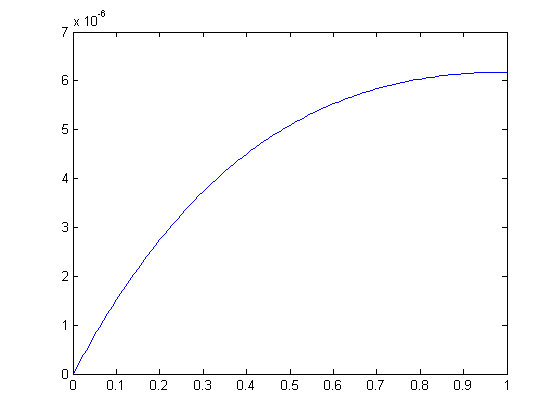
\includegraphics[width=\textwidth]{img/2-8-4c.png}
	\end{figure}
	
	The plot of $ln(E)$ is given by the red curve, while the blue curve is $ln(t)$. This shows that the accumulation of the error $E$ slows down as $t$ increases.
	
	\begin{figure}[H]
		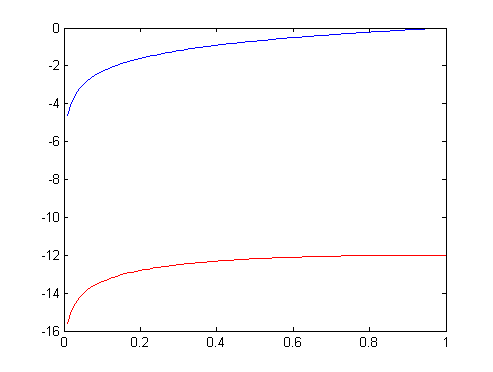
\includegraphics[width=\textwidth]{img/2-8-4c2.png}
	\end{figure}
	
	
	\subsection*{2.8.6 A}
	\begin{figure}[H]
		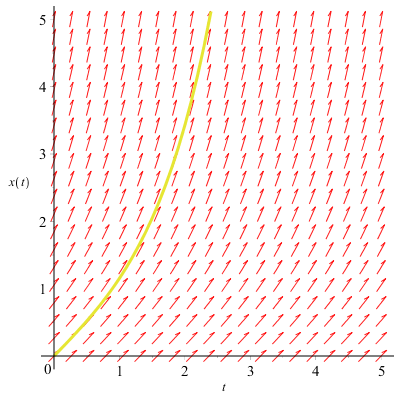
\includegraphics[width=\textwidth]{img/2-8-6a.png}
	\end{figure}
	
	\subsection*{2.8.6 B}
	Using Taylor series, $x + e^{-x} = 1 + \frac{x^2}{2} + O(x^3)$. We know that for all x, $1 \leq x + e^{-x} \leq 1 + \frac{x^2}{2}$. We then integrate them and find the lower bound $t \leq x(t)$. To find the upperbound we find a solution for $\frac{dx}{dt} = 1 + \frac{x^2}{2}$.
	
	\begin{align*}
	t &= \int \frac{2dx}{1 + (1/2)}\\
	&= \int \frac{2\sqrt{2}sec^2(u) du}{2 + 2tan^2(u)}\\
	&= \int \frac{2\sqrt{2}sec^2(u) du}{2sec^2(u)}\\
	&= \int \sqrt{2}\\
	&= \sqrt{2} tan(\frac{x}{\sqrt{2}})
	\end{align*}
	
	So the bounds would be $t \leq x(t) \leq \sqrt{2} tan(\frac{t}{\sqrt{2}}$. Therefore, $1 \leq x(1) \leq 1.208$.
	
	\subsection*{2.8.6 C} $\delta t = 0.0001$ would yield $x(1) = 1.1536$, which is correct when rounded to 3 decimal places.
	\subsection*{2.8.6 D}
	
	\begin{align*}
	&\Delta t = 1: & \hat x (1) &=  1.1536059\\
	&\Delta t = 0.1: & \hat x (1) &= 1.1536389\\
	&\Delta t = 0.01: & \hat x (1) &= 1.153639
	\end{align*}
	
	
	\subsection*{2.8.8} The exact value $x(t_1) = x(t_0) + \Delta t)$ can be expanded to $x (t_0) + \dot x(t_0) \Delta t + \frac{\ddot x(t_0) \Delta t^2}{2} + \frac{\dddot x(t_0) \Delta t^3}{6} + O(\Delta t^4)$. Let $\dot x = f(x)$, and $\ddot x = f'(x) f(x)$, and $\dddot x = f'(x)^2 f(x) + f''(x)f(x)^2$. Then we get $x_0 + f(x_0)\Delta t + \frac{f'(x_0) f(x_0) \Delta t^2}{2} + \frac{(f'(x_0)^2 f(x_0) + f''(x_0)f(x_0)^2) \Delta t^3}{6} + O(\Delta t^4)$.\\
	
	We use the same expansion to the trial step of the Improved Euler method. Let $\bar x = f(x)$ and we get $f(x_0) + f'(x_0) f(x_0) \Delta t + \frac{(f'(x_0^2 f(x_0) + f''(x_0)f(x_0)^2) \Delta t^2}{2} + O(\Delta t^3)$.\\
	
	To get $|x(t_n) - x_n|$, substitute the expansion of the trial step in $x_n$. 
	
	\begin{align*}
	|x(t_n) - x_n| &= x_0 + f(x_0)\Delta t + \frac{f'(x_0) f(x_0) \Delta t^2}{2} + \frac{(f'(x_0)^2 f(x_0) + f''(x_0)f(x_0)^2) \Delta t^3}{6} + O(\Delta t^4)\\
	& -\Bigg[ x_0 + \frac{\Delta t}{2} [f(x_0) + f(\bar x_1)] \Bigg]\\
	&= x_0 + f(x_0)\Delta t + \frac{f'(x_0) f(x_0) \Delta t^2}{2} + \frac{(f'(x_0)^2 f(x_0) + f''(x_0)f(x_0)^2) \Delta t^3}{6} + O(\Delta t^4)\\
	& -\Bigg[ x_0 + \frac{\Delta t}{2} \Bigg[2f(x_0) + f'(x_0) f(x_0) \Delta t + \frac{(f'(x_0)^2 f(x_0) + f''(x_0)f(x_0)^2) \Delta t^2}{2} + O(\Delta t^3)\Bigg] \Bigg]\\
	&=\frac{(f'(x_0)^2 f(x_0) + f''(x_0)f(x_0)^2) \Delta t^3}{6} - \frac{(f'(x_0)^2 f(x_0) + f''(x_0)f(x_0)^2) \Delta t^3}{4} + O(\Delta t^4)
	\end{align*}
	
	Therefore, the local error for the improved euler is $O(\Delta t^3)$
	
	\section*{Chapter 3}
	\subsection*{3.1.2} $\dot{x}=r-\cosh(x)$ - saddle-node bifurcation
	
	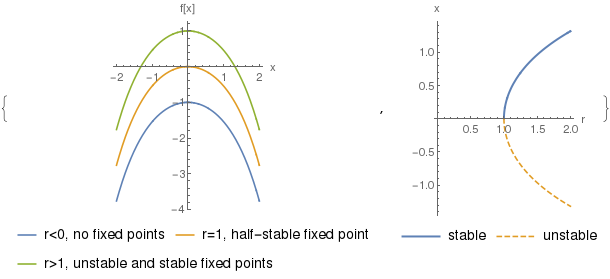
\includegraphics[width=\textwidth]{312.png}
	
	\subsection*{3.1.4} $\dot{x}=r+\frac{1}{2}x-\frac{x}{x+1}$ - transcritical bifurcation
	
	First, we get the extreme values of $g(x)=\frac{1}{2}x-\frac{x}{x+1}=\frac{x^2-x}{2x+2}$ to know where bifurcations occur.
	\begin{align*}
	g'(x) &= \frac{(x^2-x)(2)-(2x+2)(2x-1)}{(2x+2)^2}\\
	g'(x) &= \frac{x^2+2x-1}{2(x+1)^2} = 0\\
	x_{1,2} &= -1 \pm \sqrt{2} \to g(x_{1,2}) = \pm 2 - \frac{3}{2}
	\end{align*}
	Then $r$ shifts $g(x)$ up or down that makes fixed points coalesce.
	
	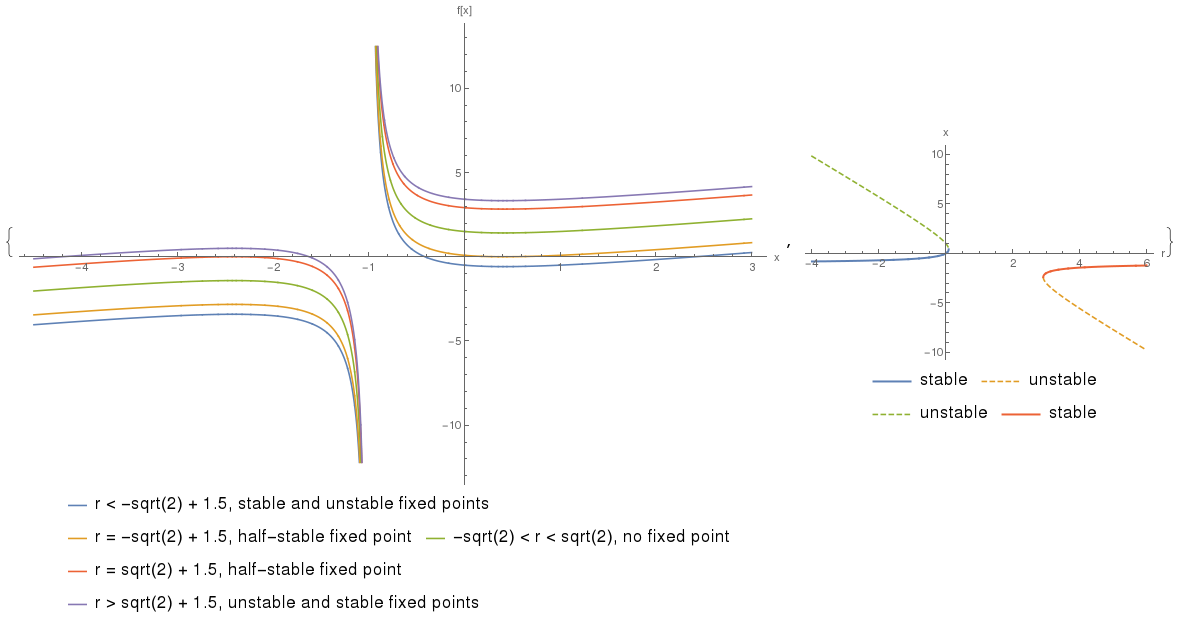
\includegraphics[width=\textwidth]{314.png}
	
	\subsection*{3.2}
	\textbf{3.2.2} Below are the plots of $\dot{x}$ vs $x$ for $\dot{x} = rx - \ln(1+x)$ for the specified values of $r$. It can be seen that the transcritical bifurcation occurs at $r=1$. The bifurcation diagram follows.
	\\
	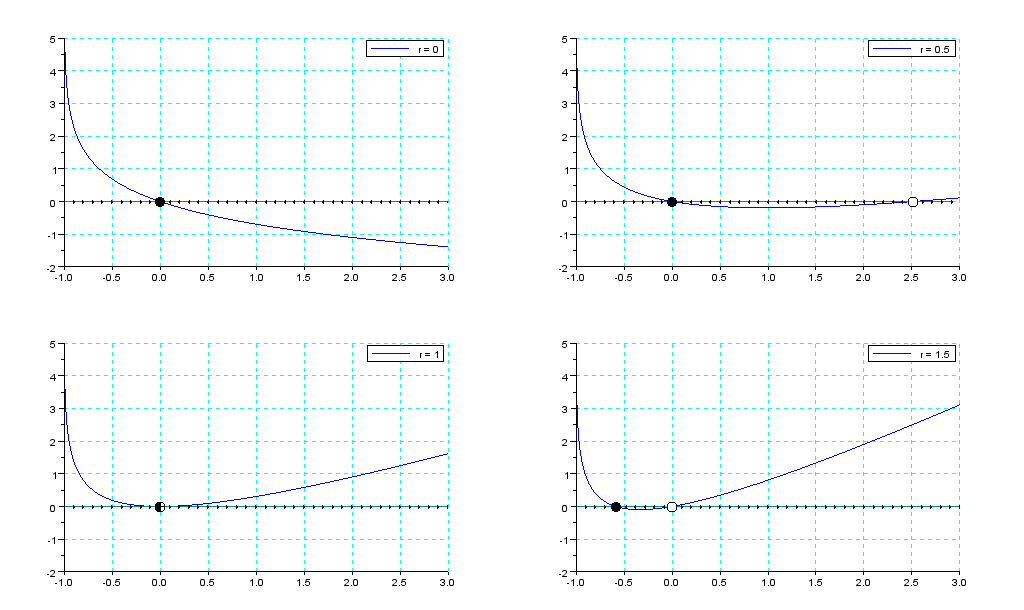
\includegraphics[width=\textwidth]{322}
	\\
	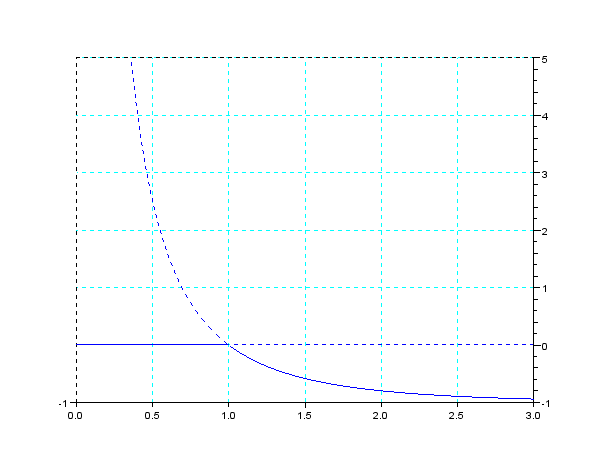
\includegraphics[width=.5\textwidth]{322r}
	
	\textbf{3.2.4} Below are the plots of $\dot{x}$ vs $x$ for $\dot{x} = x(r-e^x)$ for the specified values of $r$. It can be seen that the transcritical bifurcation occurs at $r=1$. The bifurcation diagram follows.
	\\
	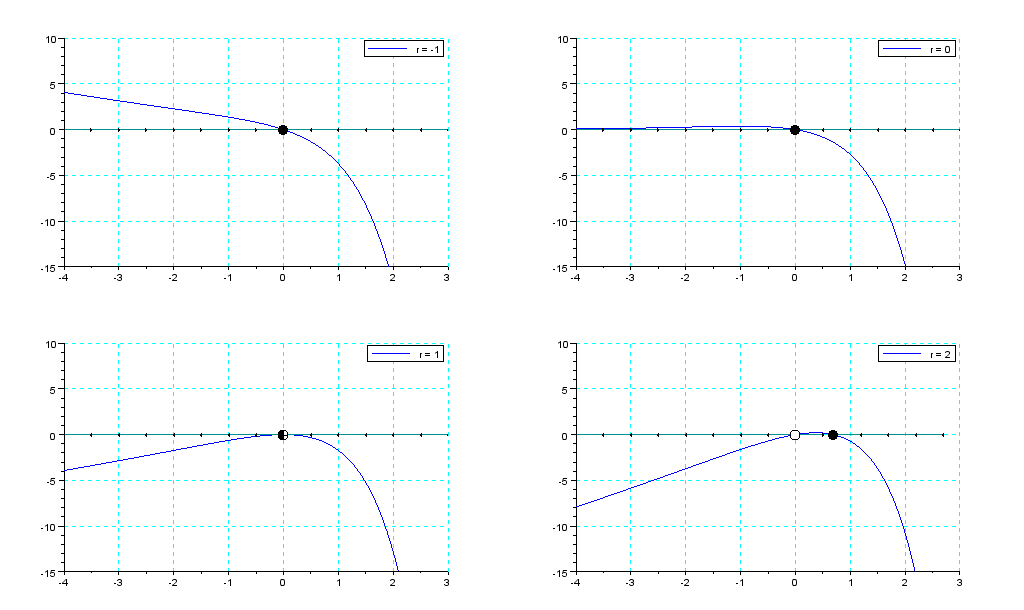
\includegraphics[width=\textwidth]{324}
	\\
	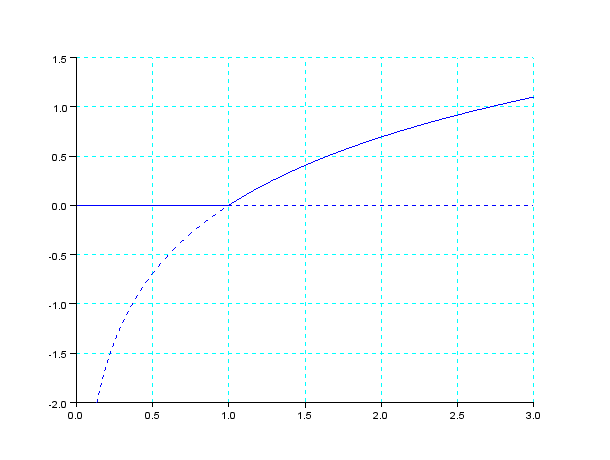
\includegraphics[width=\textwidth]{324r}
	
	%\textbf{3.2.5} The following chemical reaction system is considered:
	%\\
	%\begin{align*}
	%\ce{A + X <=>[k_1][k_-1] 2X} &and \ce{X + B ->[k_2] C}.
	%\end{align*}
	%\\ 
	\textbf{3.2.5.A} Suppose that $A$ and $B$ are kept at constant concentrations $a$ and $b$. Let $x$ be the concentration of $X$. According to the law of mass action, the rate of an elementary reaction is proportional to the product of the concentrations of the reactants. From the given reactions,
	\begin{align*}
	\dot{x} &= k_1 ax - k_{-1} x^2 - k_2 bx \\
	&= (k_1 a - k_2 b)x - k_{-1}x^2
	\end{align*}
	\\ Taking $c_1 = k_1a - k_2b$ and $c_2 = k_{-1}$ will lead to the form $\dot{x} = c_1x - c_2x^2$, where $c_1$ and $c_2$ are constant since $k_1$, $k_{-1}$, $k_2$, $a$, and $b$ are constant.
	\\ 
	
	\textbf{3.2.5.B} Substituting $x=0$ in the equation for $\dot{x}$ results to $\dot{x}=0$. Thus $x=0$ is a fixed point. Stability can be shown if the derivative of $\dot{x}$ at $x=0$ is negative. Let $f(x) = \dot{x}$. Then,
	\begin{align*}
	f(x) &= (k_1a - k_2b)x - k_{-1}x^2 \\
	f'(x) &= (k_1a - k_2b) - 2k_{-1}x \\
	f'(0) &= k_1a - k_2b
	\end{align*}
	If $k_2b > k_1a$, $f'(0) < 0$, thus $x = 0$ is a stable fixed point.
	\\
	
	Chemically, $k_2b > k_1a$ implies that $X$ is depleted faster than it is produced. Eventually, $X$ will run out, that is, $x = 0$. Once this happens, $x$ will remain at $0$ since $X$ is produced by using $X$.
	
	\subsection*{3.3.2 A} Assume $\dot P = 0$ and $\dot D = 0$. From $\gamma_1(ED-P) = 0$, we get $P = ED$.
	
	\begin{align*}
	0 &= \gamma_2(\lambda + 1 - D - \lambda EP)\\
	D &= \lambda + 1 - \lambda EP\\
	&= \lambda + 1 - \lambda E^2 D\\
	&= \cfrac{\lambda  +  1}{1 + \lambda E^2}\\
	\end{align*}
	
	Substitute D,
	
	\begin{align*}
	P &= \frac{E(\lambda  +  1)}{1 + \lambda E^2}\\
	\dot E &= \kappa(P - E)\\
	&= \kappa(\frac{E(\lambda  +  1)}{1 + \lambda E^2} - E)\\
	&= \lambda E\kappa(\cfrac{1-E^2}{1 +  \lambda E^2})\\
	\end{align*}
	
	\subsection*{3.3.2 B} Solving for $\dot E = 0$, the fixed points are -1, 0, and 1 when $\lambda \neq 0$, and all E if $\lambda = 0$.
	
	
	\subsection*{3.3.2 C} To test the stability of the fixed points, we get the derivative of $\dot E$.
	
	\begin{equation*}
	f'(E) = \lambda\kappa \frac{1 - (\lambda + 3)E^2 - \lambda E^4}{(1 + \lambda E^2)^2}
	\end{equation*}
	
	At $E^* = 0$, $f'(0) = \lambda \kappa$. Therefore, it is stable when $\lambda < 0$, and unstable when $\lambda > 0$.\\
	
	At $E^* = 1$ and $E^* = -1$,
	\begin{equation*}
	f'(1) = f'(-1) = \frac{-2\lambda \kappa}{1 + \lambda}    
	\end{equation*}
	
	Therefore they are stable when $\lambda > 0$ and $\lambda < -1$, and unstable when $-1 < \lambda < 0$. The diagram is shown below. 
	
	\begin{figure}[H]
		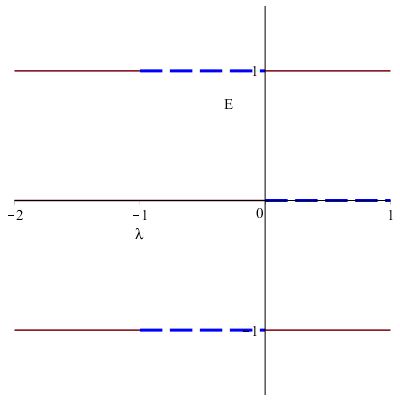
\includegraphics[width=\textwidth]{img/3-3-2c.png}
	\end{figure}
	
	\subsection*{3.4.2} $\dot{x} = rx - \sinh(x)$, supercritical pitchfork bifurcation
	
	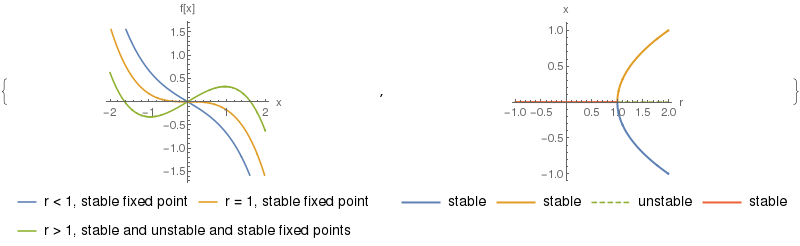
\includegraphics[width=\textwidth]{342.png}
	
	\subsection*{3.4.4} $\dot{x} = x + \frac{rx}{1+x^2}$, subcritical pitchfork bifurcation
	
	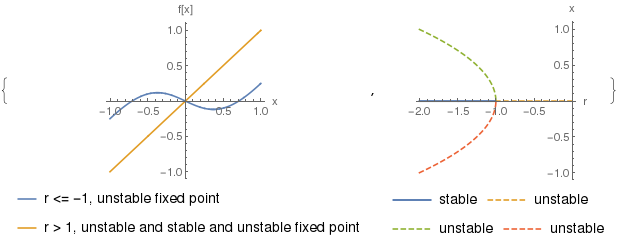
\includegraphics[width=\textwidth]{344.png}
	
	\subsection*{3.4.6} $\dot{x} = rx-\frac{x}{1+x}$, transcritical bifurcation
	
	
	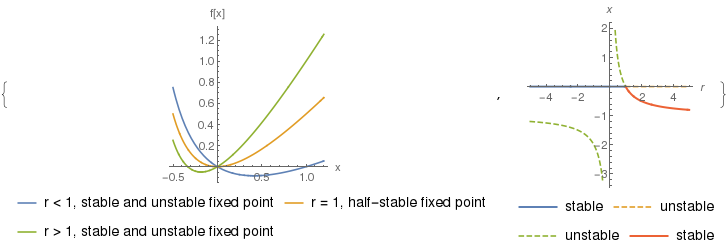
\includegraphics[width=\textwidth]{346.png}
	
	\subsection*{3.4.8} $\dot{x} = x\left(r-\frac{1}{1+x^2}\right)$, transcritical bifurcation
	
	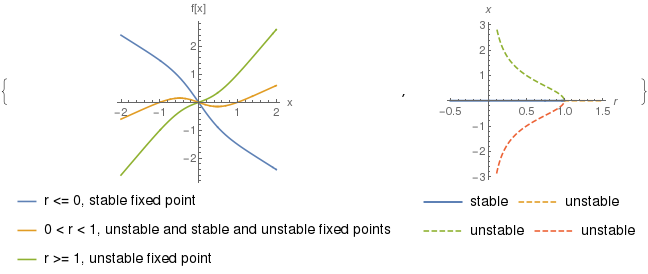
\includegraphics[width=\textwidth]{348.png}
	
	\subsection*{3.4.14}
	\textbf{A.} Let $\dot{x}=rx+x^3-x^5$ and $\ddot{a}=r+3x^2-5x^4$.
	The fixed points as a function of $r$ are given by
	\begin{align*}
	0 &= x\left(r+x^2-x^4\right)\\
	0 &= x \left(x+\frac{\sqrt{1-\sqrt{1+4r}}}{2}\right) \left(x-\frac{\sqrt{1-\sqrt{1+4r}}}{2}\right) \left(x+\frac{\sqrt{1+\sqrt{1+4r}}}{2}\right) \left(x-\frac{\sqrt{1-\sqrt{1+4r}}}{2}\right)\\
	x &=0, \quad x = \pm\frac{\sqrt{1+\sqrt{1+4r}}}{2}, \quad x = \pm\frac{\sqrt{1-\sqrt{1+4r}}}{2}
	\end{align*}
	
	\textbf{B.} The vector field and bifurcation diagram is given below:
	
	
	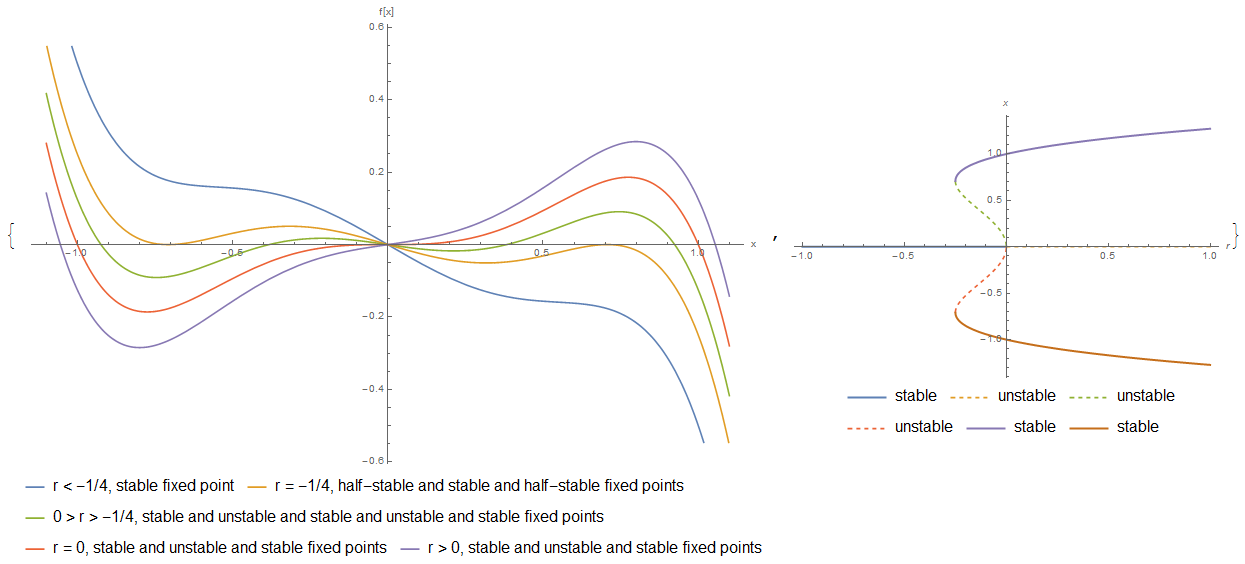
\includegraphics[width=\textwidth]{3414.png}
	
	
	\textbf{C.} The values of $r_s=0, -\frac{1}{4}$ are the critical points for saddle node bifurcations by setting $\dot{x}$ and $\ddot{x}$ equal to zero.
	
	\subsection*{3.4.16}
	\textbf{A.} $\dot{x}=r-x^2$
	\begin{align*}
	-V(x) &= rx-\frac{1}{3}x^3\\
	V(x)&=\frac{1}{3}x^3-rx
	\end{align*}
	
	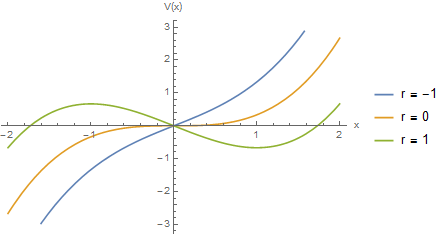
\includegraphics[width=\textwidth]{3416a.png}
	
	\textbf{B.} $\dot{x}=rx-x^2$
	\begin{align*}
	-V(x) &= \frac{r}{2}x^2-\frac{1}{3}x^3\\
	V(x)&=\frac{1}{3}x^3-\frac{r}{2}x^2
	\end{align*}
	
	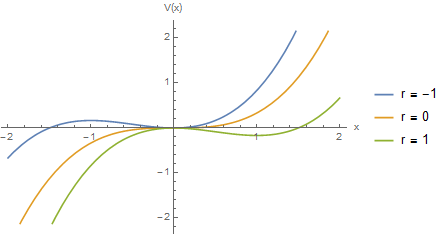
\includegraphics[width=\textwidth]{3416b.png}
	
	\textbf{C.} $\dot{x}=rx+x^3-x^5$
	\begin{align*}
	-V(x) &= \frac{r}{2}x^2+\frac{1}{4}x^4-\frac{1}{6}x^6\\
	V(x)&=\frac{1}{6}x^6-\frac{1}{4}x^4-\frac{1}{2}x^2
	\end{align*}
	
	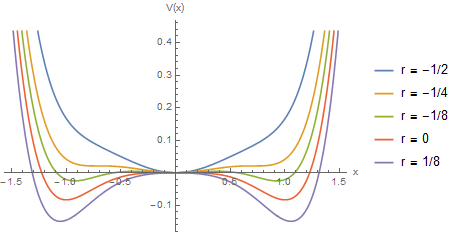
\includegraphics[width=\textwidth]{3416c.png}
	
	\subsection*{3.5.2}
	Consider the equation $b\dot{\phi} = mg\sin\phi (\frac{r \omega^2}{g}\cos \phi -1)$. Finding the fixed points, $b\dot{\phi} = 0$ either $mg\sin\phi = 0$ or $\frac{r \omega^2}{g}\cos \phi = 1$. The first case implies that $\sin \phi = 0$, that is, $\phi = \pm \pi$. Similarly, the second case implies that $\cos \phi = \frac{g}{r \omega^2}$. It follows that $\phi = \pm \cos^{-1} \frac{g}{r \omega^2}$.\\
	Thus, the fixed points are 0, $\pm \pi$, $\pm \cos^{-1}\frac{g}{r \omega^2}$.\\
	To check for stability we take $b\ddot{\phi} = mr\omega^2 \cos^2\phi - mr\omega^2\sin^2\phi - mg\cos\phi$. Taking the values of $\ddot{\phi}$ at the fixed points,\\
	\begin{align*}
	\ddot{\phi}(0) &= mr\omega^2 - mg\\  
	\ddot{\phi}(0) &> 0 \quad, if \quad mr\omega^2 > mg, \rightarrow \gamma = \frac{r\omega^2}{g} > 1\\ 
	\ddot{\phi}(0) &< 0 \quad, if \quad mr\omega^2 < mg, \rightarrow \gamma = \frac{r\omega^2}{g} < 1
	\end{align*}
	Thus, 0 is a stable fixed point if $\gamma < 1$ and it is unstable if $\gamma > 1$. Similarly,
	\begin{align*}
	\ddot{\phi}(\pm \pi) &= mr\omega^2 + mg\\
	&> 0, \textmd{since  all quantities are positive.}\\
	\ddot{\phi}(\cos^{-1} (\frac{g}{r\omega^2})) &= \ddot{\phi}(\cos^{-1} (\frac{1}{\gamma}))\\
	&= mr\omega^2(\cos^2(\cos^{-1}(\frac{1}{\gamma}))) - mr\omega^2(\sin^2(\cos^{-1}(\frac{1}{\gamma})) - mg\cos(\cos^{-1}(\frac{1}{\gamma}))\\
	&= \frac{mr\omega^2}{\gamma^2} - \frac{mg}{\gamma} - mr\omega^2(\frac{r^2\omega^4 - g^2}{r^2\omega^4})\\
	&= \frac{mg}{\gamma} - \frac{mg}{\gamma} - mr\omega^2 (1 - \frac{1}{\gamma^2})\\
	&=mr\omega^2 (1 - \frac{1}{\gamma^2}).\\
	\gamma &> 1 \quad \rightarrow \quad \frac{1}{\gamma^2} < 1 \quad \rightarrow \quad \ddot{\phi} < 0.
	\end{align*}
	Thus $\ddot{\phi}(\cos^{-1} (\frac{1}{\gamma}))$ is a stable fixed point when $\gamma > 1$.\\
	This shows that the given bifurcation diagram is correct.
	
	\subsection*{3.5.4}
	\textbf{A.} Expressing Newton's law, $m\ddot{x} = -bx -k\Delta x \cos \theta$, in terms of the given parameters, we get $m\ddot{x} + b\dot{x} + kx (1- \frac{L_o}{\sqrt{h^2 + k^2}}) = 0$.
	
	\textbf{B.} To get the fixed points of the associated first order system we have
	\begin{align*}
	-k\left(1-\frac{L_0}{\sqrt{h^2+k^2}}\right)x&=0 \to x=0
	\end{align*}
	
	\textbf{C.} Assuming $k>0, m>0$, the fixed point $x=0$ is half-stable.
	
	\textbf{D.} To nondimensionalize the equation, one can do the following:
	\begin{align*}
	\ddot{x} + \frac{b}{m}\dot{x} + \frac{k}{m}\left(1-\frac{L_0}{\sqrt{h^2+k^2}}\right)x&=0
	\end{align*}
	
	Let $\tau = mt/b$, $x'=dx/d\tau$ and $\gamma=\frac{k}{m}\left(1-\frac{L_0}{\sqrt{h^2+k^2}}\right)$ to yield
	\begin{align*}
	\frac{m^2}{b^2}x'' + x' + \gamma x=0
	\end{align*}
	
	For $x''$ to be negligible, the system should have $\frac{m^2}{b^2}<<1 \to m^2 << b^2$, which means $m$ is considered negligible under a large damping.
	
	\subsection*{3.5.6}
	
	\textbf{A.} Given a linear second-order differential equation $\epsilon \ddot{x} + \dot{x} + x = 0$, the solution is given by $x(t) = A\mathbf{e}^{\lambda_1} + B \mathbf{e}^{\lambda_2}$ where $\lambda_{1,2}$ are the roots of the equation $\epsilon \lambda^2 + \lambda + 1 =0$. Finding $lambda_{1,2}$ is achieved using the quadratic formula
	
	\begin{align*}
	\lambda_{1,2} = \frac{1}{2\epsilon}\left(-1\pm\sqrt{1-4\epsilon}\right)
	\end{align*}
	
	Therefore the general solution is
	\begin{align*}
	x(t)\to A e^{\frac{\left(-\sqrt{1-4 e}-1\right) t}{2 e}}+B e^{\frac{\left(\sqrt{1-4 e}-1\right) t}{2 e}}
	\end{align*}
	
	Using the initial conditions $x(0)=1, \dot{x}(0)=0$, we can find the constants. Finally, the specific solution is given by:
	\begin{align*}
	x(t)=\frac{\sqrt{1-4 \epsilon}\: e^{\frac{\left(-\sqrt{1-4 \epsilon}-1\right) t}{2 \epsilon}}+\sqrt{1-4 \epsilon}\: e^{\frac{\left(\sqrt{1-4 \epsilon}-1\right) t}{2 \epsilon}}-e^{\frac{\left(-\sqrt{1-4 \epsilon}-1\right) t}{2 \epsilon}}+e^{\frac{\left(\sqrt{1-4 \epsilon}-1\right) t}{2 \epsilon}}}{2 \sqrt{1-4 \epsilon}}
	\end{align*}
	
	\textbf{B.} Convert the second-order equation to system of first-order differential equations:
	
	\begin{align*}
	\dot{x} &= y\\
	\dot{y} &= \frac{-1}{\epsilon}\left(x+y\right)
	\end{align*}
	
	Now if $\epsilon<<1$, the two widely separated time scales are $\dot{x}$, evolving slowly and $\dot{y}$, evolving very fast.
	
	\textbf{C.} The graph for $\epsilon=0.001$ is shown below:
	
	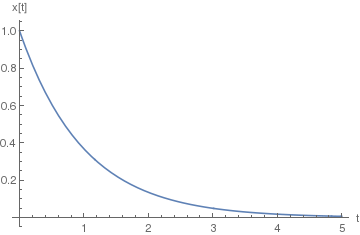
\includegraphics[width=.5\textwidth]{356}
	
	\textbf{D.}
	Note that the graph above is almost similar to $\hat{x}(t) = \mathbf{e}^{-t}$. As long as $\epsilon$ is very small, the singular limit is a good alternative. Nondimensionalizing the equation (let $\tau=\epsilon t$) leads to $\epsilon^2 x'' + x' +x = 0$ and to neglect the second-order term we must let $\epsilon^2 << 1$, further supporting the validity of replacing it with the singular limit.
	
	
	\subsection*{3.6.2 A} $\dot x = h + rx - x^2$
	
	\begin{figure}[H]
		\centering
		\subfloat[h $<$ 0]
		{{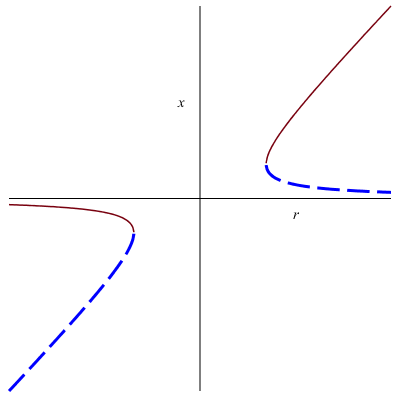
\includegraphics[width=5cm]{img/3-6-2ahn.png} }}%
		\qquad
		\subfloat[h = 0]
		{{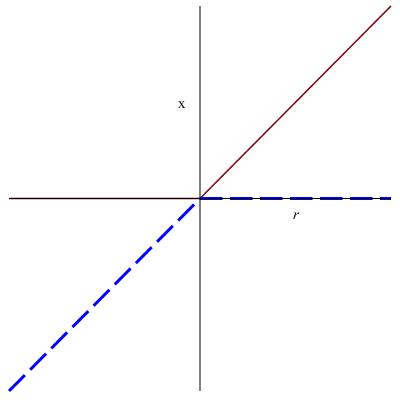
\includegraphics[width=5cm]{img/3-6-2ah0.png} }}%
		\qquad
		\subfloat[h $>$ 0]
		{{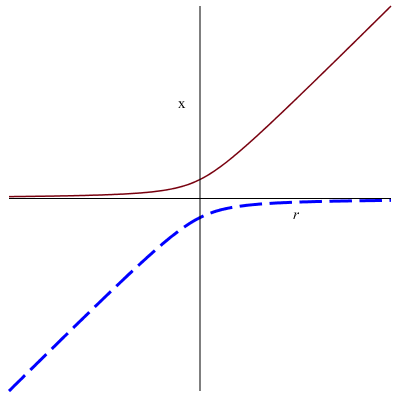
\includegraphics[width=5cm]{img/3-6-2ahp.png} }}%
		\caption{}%
		\label{fig:example}%
	\end{figure}
	
	\subsection*{3.6.2 B} Using the discriminant $r^2 + 4h$, we can find the curve that separates the region. Note that there are two fixed points when it is positive, no fixed point when it is negative, and one fixed point when it is zero. There is a transcritical bifurcation when r = 0 and h = 0, and saddle node bifurcation when $(r, h)$ is on the curve but is not $(0,0)$.
	
	\begin{figure}[H]
		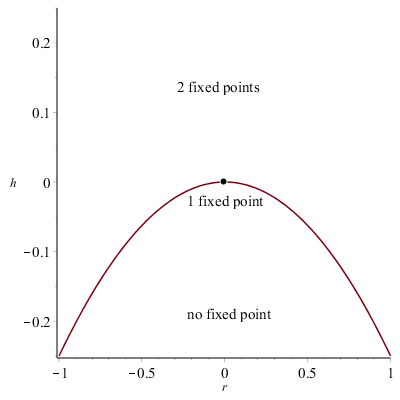
\includegraphics[width=\textwidth]{img/3-6-2b.png}
	\end{figure}
	
	\subsection*{3.6.2 C} There are two regions, one above and one below the curve $h = \frac{-r^2}{4}$.
	
	\begin{figure}[H]
		\centering
		\subfloat[above the curve]
		{{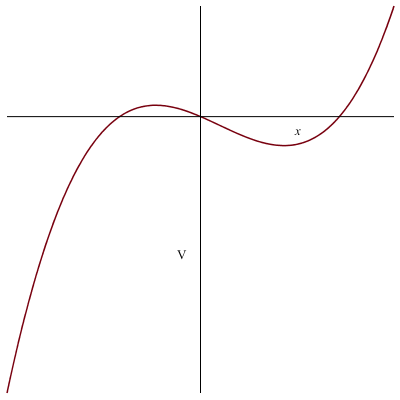
\includegraphics[width=5cm]{img/3-6-2c.png} }}%
		\qquad
		\subfloat[below the curve]
		{{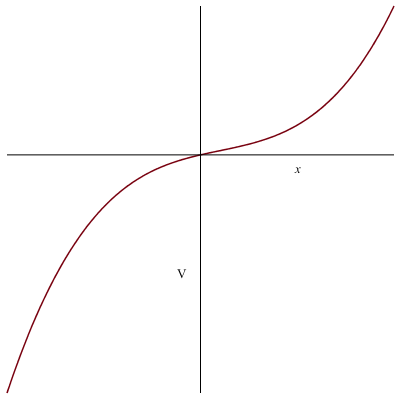
\includegraphics[width=5cm]{img/3-6-2c2.png} }}%
		\qquad
		\caption{}%
		\label{fig:example}%
	\end{figure}
	
	
	\subsection*{3.6.4} If you add a small imperfection in a system with a saddle node bifurcation, the saddle node will just adjust with the difference of $h$, where $h$ is just the imperfection. Basically, it will seem like you added or subtracted a small value from 
	
	\subsection*{3.6.6 A}
	The roots of the Landau equation are $A^* = 0, \pm \sqrt{\frac{\varepsilon}{g}}$. Assuming that $\beta = 0.5$, then $A^* \propto \sqrt{ \frac {\epsilon}{g}}$. So the Landau equation predicts the constant of proportionality of the power law.
	
	\subsection*{3.6.6 B}
	\begin{align*}
	\tau \dot A &= \varepsilon A - gA^3 - kA^5\\
	0 &= \varepsilon A - kA^5\\
	0 &= A(\varepsilon - kA^4)\\
	A^* &= \Big(\frac{\varepsilon}{k}\Big)^{\frac{1}{4}}
	\end{align*}
	
	\subsection*{3.6.6 C}
	\begin{figure}[H]
		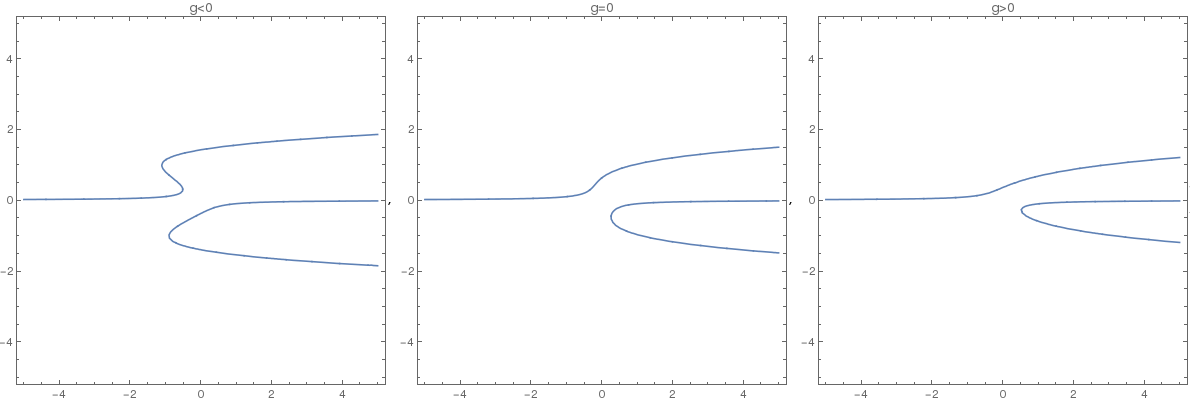
\includegraphics[width=\textwidth]{img/3-6-6c.png}
	\end{figure}
	
	\subsection*{3.6.6 D}
	When $\varepsilon_f$ is larger, the rate of change also gets larger. The sytem approaches a fixed point in longer time as $\varepsilon_f$ gets small. This can be seen in the graph below
	\begin{figure}[H]
		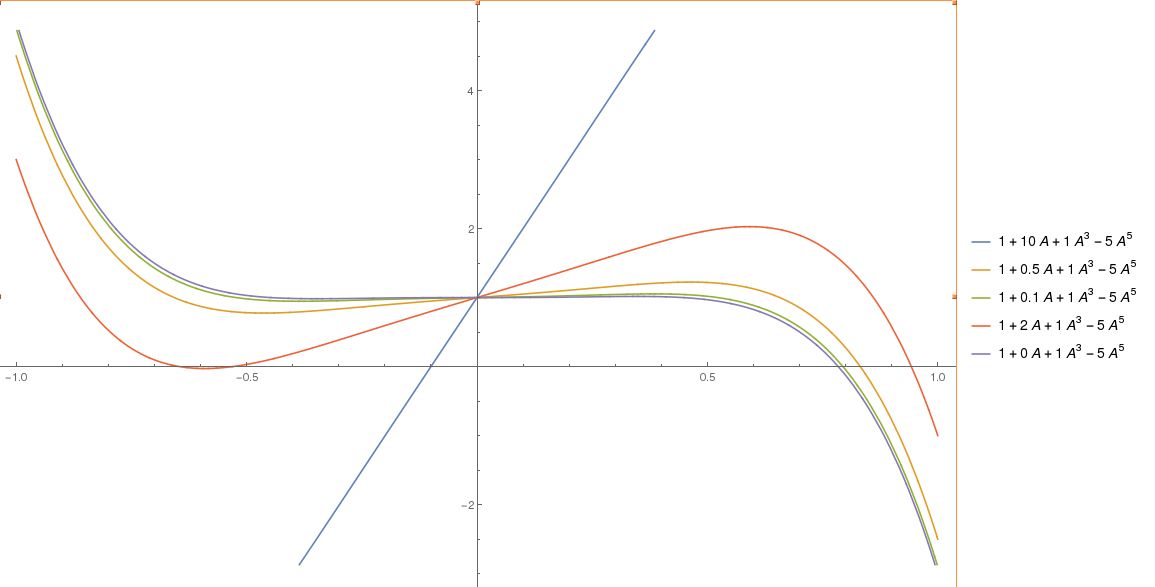
\includegraphics[width=\textwidth]{img/3-6-6d.png}
	\end{figure}
	
	\subsection*{3.7.2}
	\textbf{A.} The graph of $r(x)$ and $k(x)$ is given below:
	
	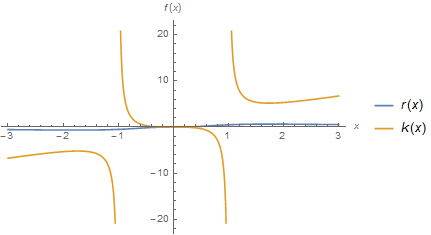
\includegraphics[width=\textwidth]{372a.png}
	
	\textbf{B.} The limiting behaviors are given by
	\begin{align*}
	\lim_{x \to 1}r(x),k(x)&=\frac{1}{2},\infty\\
	\lim_{x \to \infty}r(x),k(x)&=0, \infty
	\end{align*}
	
	\textbf{C.} To find the cusp in the graph parametrized by $\left(k(x),r(x)\right)$, we should find $x$ such that
	\begin{align*}
	\frac{dk}{dx}&=\frac{dr}{dx}=0\\
	\frac{dk}{dx}&=\frac{2x^2\left(x^2-3\right)}{\left(x^2-1\right)^2}\\
	\frac{dr}{dx}&=\frac{2x^2\left(x^2-3\right)}{\left(x^2+1\right)^3}\\
	x=0 \quad &\text{or} \quad x=\pm\sqrt{3}
	\end{align*}
	Since $x>1$ is assumed, we pick $x_0=\sqrt{3}$ and the cusp point is $\left(r(x_0),k(x_0)\right)=\left(\frac{3}{8}\sqrt{3},3\sqrt{3}\right)$.
	
	\subsection*{3.7.4}
	\textbf{A.}For the improved model of a fishery, we have
	\begin{align*}
	\dot{N}=rn\left(1-\frac{N}{K}\right)-H\frac{N}{A+N}
	\end{align*}
	The parameter $A$ measures the diffusion rate of population. If $A=0$, the fish are harvested at a constant rate. If $A>0$, the harvest rate is less than expected because the population are more diffused.
	\\
	
	\textbf{B.} We let $x=\frac{N}{k}, \dot{N}=k\frac{dx}{dt}$. Then we have
	\begin{align*}
	k \frac{dx}{dt} &= rkx(1-x)-H \left(\frac{kx}{A+kx}\right)\\
	\frac{1}{r}\frac{dx}{dt}&=x(1-x)-\frac{Hx}{rk}\left(\frac{1}{\frac{A}{k}+x}\right)
	\end{align*}
	Furthermore, we let $\tau=rt, \frac{d\tau}{dt}=r, h=\frac{H}{rk}$ and $a=\frac{A}{k}$. Since $\frac{dx}{d\tau}=\frac{dx}{dt}\frac{dt}{d\tau}=\frac{1}{r}\frac{dx}{dt}$, we have
	\begin{align*}
	\frac{dx}{d\tau}=x(1-x)-h\left(\frac{x}{a+x}\right)
	\end{align*}
	which is the required dimensionless form.
	
	\textbf{C.} We need to find the fixed points $x$ as a function of $a>0$ and $h>0$.
	\begin{align*}
	0 &= x(1-x) - \frac{hx}{a+x}\\
	0 &= x - x^2 - \frac{hx}{a+x}\\
	0 &= \frac{ax + x^2 -ax^2 -x^3 -hx}{a+x}\\
	0 &= \frac{(a-h)x + (1-a)x^2 - x^3}{a+x}\\
	0 &= x \left[(a-h) + (1-a)x - x^2\right]\\
	0 &= -x \left[x^2 - (1-a)x - (a-h)\right]\\
	x = 0 \quad &\text{or} \quad x = \frac{1}{2}\left(1-a \pm \sqrt{(1-a)^2+4(a-h)}\right)\\
	x_1 = 0 \quad &\text{or} \quad x_{2,3} = \frac{1}{2}\left(1-a \pm \sqrt{(a+1)^2-4h}\right)
	\end{align*}
	
	We let $\Delta = (a+1)^2-4h$. Therefore we have a fixed point if $\Delta < 0$, two fixed points if $\Delta = 0$ and three fixed points if $\Delta > 0$. To classify the fixed points, find the values of their second derivatives:
	\begin{align}
	\ddot{x} &= 1 - 2x + \frac{ah}{(a+x)^2}\\
	\ddot{x} | _{x_1} &= 1 - \frac{h}{a} \quad
	\begin{cases}
	\text{stable}, h<a\\
	\text{half-stable}, h=a\\
	\text{unstable}, h>a
	\end{cases}
	\\
	\ddot{x} | _{x_2} &= -\frac{4 a h}{\left(-\sqrt{(a+1)^2-4 h}+a+1\right)^2}+\sqrt{(a+1)^2-4 h}+a \\
	&:
	\begin{cases}
	\text{stable}, h=\frac{1}{4}(a+1)^2, a\geq 1\\
	\text{half-stable}, \left(h=a, 0<a<1\right) \text{or} \left(h=\frac{1}{4}(a+1)^2, 0 < a < 1 \text{ or } a > 1\right)
	\end{cases}
	\\
	\ddot{x} | _{x_3} &= -\frac{4 a h}{\left(\sqrt{(a+1)^2-4 h}+a+1\right)^2}-\sqrt{(a+1)^2-4 h}+a\\
	&:
	\begin{cases}
	\text{stable}, h=\frac{1}{4}(a+1)^2, 0<a\geq 1\\
	\text{half-stable}, \left(h=a, a>1\right) \text{ or } \left(h=\frac{1}{4}(a+1)^2, 0<a<1 \text{ or } a>1\right)
	\end{cases}
	\end{align}
	
	\textbf{D.} The dynamics of the fixed point $x=0$ is explained by equation (2). Indeed, bifurcation occurs at $h=a$ where the fixed point changes its stability. This is a saddle-node birfurcation.
	
	\textbf{E.} For fixed points $x_{2,3}$, bifurcation occurs when they lose stability. Statements (4) and (6) justifies this situation, then $h=\frac{1}{4}(a+1)^2$, for $a<1$. Therefore $a_c=1$.
	
	\textbf{F.} To plot the stability diagram in $(a,h)$ parameter space, we find $a(x)$ and $h(x)$ where saddle node bifurcation occurs.
	\begin{align}
	x(1-x)&=\frac{hx}{a+x}\\ \frac{d}{dx}\left[x(1-x)\right]&=\frac{d}{dx}\left[\frac{hx}{a+x}\right]\\ 1-2x&=\frac{h(a+x)-hx}{(a+x)^2}=\frac{ha}{(a+x)^2}\\
	h&=\frac{1}{a}(1-2x)(a+x)^2
	\end{align}
	From equation (7) and (10), we have
	\begin{align}
	x(1-x) &= \frac{x(1-2x)(a+x)}{a}\\
	ax-ax^2 &= ax+x^2-2ax^2-2x^3\\
	0 &= x^2\left[a-(1-2x)\right]\\
	x &= 0 \text{ or } a = 1-2x\\
	h &= \frac{1-2x}{1-2x}(1-2x+x)^2\\
	h &= (1-x)^2
	\end{align}
	Therefore, the parameter space is given by $\left[a(x),h(x)\right]=\left[(1-2x),(1-x)^2\right]$ which simplifies to $h=
	\frac{1}{4}(a+1)^2$. The limiting behaviors and parametric plot are given by
	\begin{align*}
	\lim_{x->-\infty}a(x),h(x) &= \infty,\infty\\
	\lim_{x->0}a(x),h(x) &= 1,1\\
	\lim_{x->\infty}a(x),h(x) &= -\infty,-\infty
	\end{align*}
	
	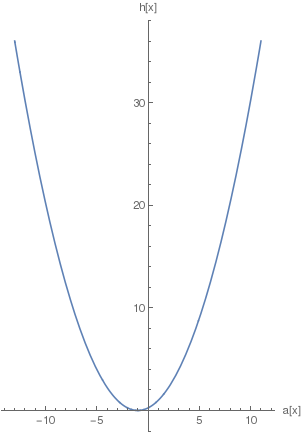
\includegraphics[width=.5\textwidth]{374b.png}
	
	At the bottom of parabola we have a fixed point, since $\Delta<0$, at the parabola we have 2 fixed points $(\Delta=0)$ and above we have three $(\Delta>0)$.
	
	\section*{Chapter 4}
	\subsection*{4.1}
	\textbf{4.1.2}\\
	The fixed points of $\dot{\theta} = 1 + 2\cos\theta$ are given by $\cos \theta = -\frac{1}{2}$, that is, $\theta = \frac{2\pi}{3}, \frac{4\pi}{3} + 2\pi k,  \forall k \in \mathbb{Z}$.
	\\
	Let $f(\theta)$ = $\dot{\theta}$, then $f'(\theta) = -2\sin\theta$.\\
	$f'(\frac{2\pi}{3}  + 2\pi k) = -\sqrt{3}, \forall k \in \mathbb{Z}$. Thus it is stable.\\
	$f'(\frac{4\pi}{3}  + 2\pi k) = \sqrt{3},  \forall k \in \mathbb{Z}$. Thus it is unstable.\\
	%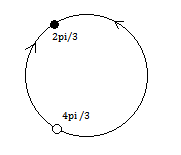
\includegraphics[width=\textwidth]{412.png}
	
	\textbf{4.1.8.A}\\
	Given $-\frac{dV}{d\theta} = \dot{\theta} =\cos\theta$, the potential is given by $V(\theta) = -\sin\theta$.\\
	Since $V(\theta + 2\pi k) = -\sin(\theta + 2\pi k) = -\sin(\theta) = V(\theta)$, $V$ is well-defined for all points on the circle.
	\\
	
	\textbf{4.1.8.B}\\
	Given $-\frac{dV}{d\theta} = \dot{\theta} =1$, the potential is given by $V(\theta) = -\theta$.\\
	Consider $\theta = 0$. Then $V(\theta) = V(0) = 0$ and $V(\theta + 2\pi) = V(2\pi) = -2\pi$. This shows that $V(\theta) \neq V(\theta + 2k\pi), \forall k \in \mathbb{Z}$. Thus, V is not well-defined on the circle.
	\\
	
	\textbf{4.1.8.C}\\
	$\dot{\theta} = f(\theta)$ has a single-valued potential when $V(\theta) = V(\theta + 2k\pi), \forall k \in \mathbb{Z}$.
	
	\subsection*{4.2.1} To compute it using common sense, we simply find the least common multiple of the durations, which in this case is equal to 12.\\
	
	To compute using the method, we just adapt the logic that the bells are oscillating uniformly. Then we can use the equation in Example 4.2.1 in Nonlinear Dynamics and Chaos (Strogatz).\\
	
	\begin{align*}
	T_{min} &= \Bigg(\frac{1}{T_1} - \frac{1}{T_2}\Bigg)^{-1}\\
	T_{min} &= \Bigg(\frac{1}{3} - \frac{1}{4}\Bigg)^{-1}\\
	T_{min} &= 12
	\end{align*}
	\\
	\subsection*{4.2.2 A} The period of modulation is $2\pi$ as can be seen in the graph.
	
	\begin{figure}[H]
		\centering
		\subfloat[]
		{{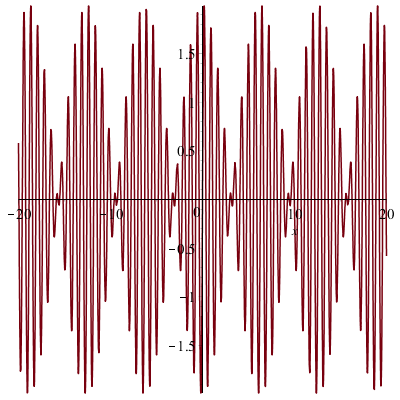
\includegraphics[width=5cm]{img/4-2-2.png} }}%
		\qquad
		\subfloat[]
		{{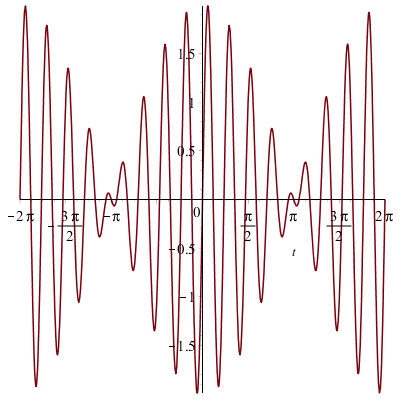
\includegraphics[width=5cm]{img/4-2-2a.png} }}%
		\caption{}%
		\label{fig:example}%
	\end{figure}
	
	\subsection*{4.2.2 B}
	
	\begin{align*}
	sin(8t) + sin(9t) &= 2sin\Bigg(\frac{8t + 9t}{2}\Bigg)cos\Bigg(\frac{8t - 9t}{2}\Bigg)\\
	&= 2sin\Bigg(\frac{17t}{2}\Bigg)cos\Bigg(\frac{-t}{2}\Bigg)\\
	&= 2sin\Bigg(\frac{17t}{2}\Bigg)cos\Bigg(\frac{t}{2}\Bigg)\\
	\end{align*}
	\\
	
	$sin(\frac{17t}{2})$ has a period of $\frac{2\pi}{17}$, while $cos(\frac{t}{2})$ has a period $2\pi$. The least common multiple is $2\pi$, and so the period is $2\pi$.
	
	\subsection*{4.3.6}
	The graph of $\dot{\theta}=\mu + \sin(\theta) + \cos(2\theta)$ is given below.
	
	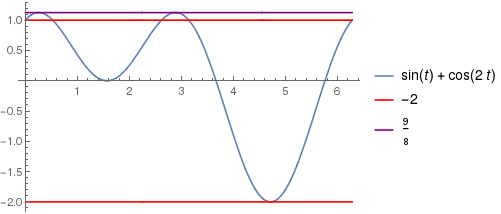
\includegraphics[width=\textwidth]{436.png}
	
	
	The critical points of $f(\theta)=\sin(\theta)+\cos(2\theta)$ are listed in the table below.
	
	\begin{table*}[h!]
		\centering
		\begin{tabular}{c | c}
			$\theta$ & $f(\theta)$\\
			\hline
			$0$ & $1$ \\
			$2\tan^{-1}\left(4-\sqrt{15}\right)$ & $9/8$ \\
			$\pi/2$ & $0$ \\
			$2\tan^{-1}\left(4+\sqrt{15}\right)$ & $9/8$ \\
			$7\pi/6$ & 0\\
			$3\pi/2$ & $-2$ \\
			$11\pi/6$ & 0\\
			$2\pi$ & $1$
		\end{tabular}
	\end{table*}
	
	Using the table and graph given, we can get the bifurcation values for $\mu$ and their phase portraits and vector field:
	\begin{table*}[h!]
		\centering
		\begin{tabular}{c | c}
			Range & No of fixed points\\
			\hline
			$u<-9/8$ & 0\\
			$\mathbf{u=-9/8}$ & 2\\
			$-1 > u > -9/8$ & 4\\
			$\mathbf{u=-1}$ & 5\\
			$0>u>-1$ & 4\\
			$\mathbf{u=0}$ & 3\\
			$0<u<2$ & 2\\
			$\mathbf{u=2}$ & 1\\
			$u>2$ & 0
		\end{tabular}
	\end{table*}
	
	
	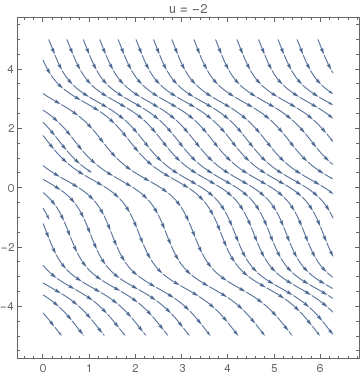
\includegraphics[width=.7\textwidth]{436a.png}
	
	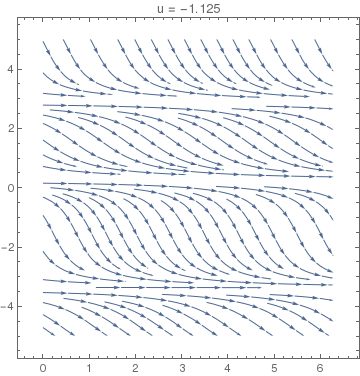
\includegraphics[width=.7\textwidth]{436b.png}
	
	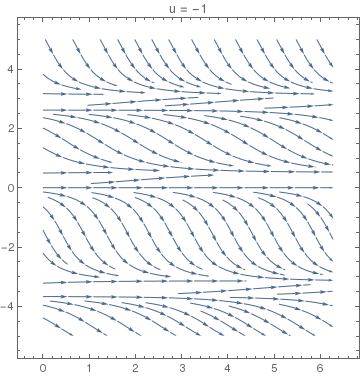
\includegraphics[width=.7\textwidth]{436c.png}
	
	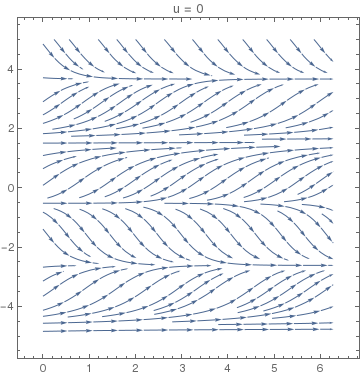
\includegraphics[width=.7\textwidth]{436d.png}
	
	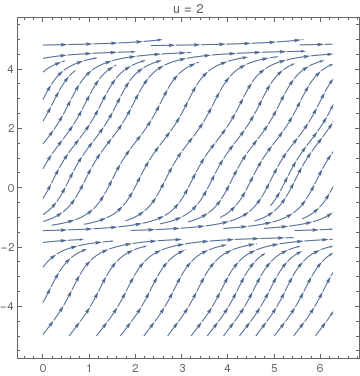
\includegraphics[width=.7\textwidth]{436e.png}
	
	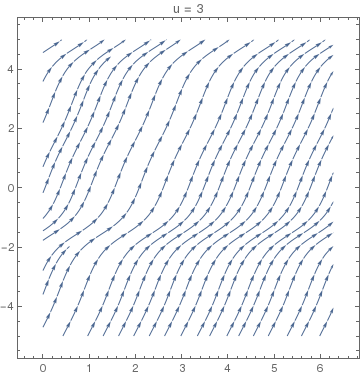
\includegraphics[width=.7\textwidth]{436f.png}
	
	
	All are just saddle-node bifurcations.
	
	\subsection*{4.3.9}
	\textbf{A.} Let $x=r^au, t=r^b\tau$ where $u,\tau \in O(1)$. Then the following must hold:
	
	\begin{align*}
	\frac{dx}{dt}&=r^a\frac{du}{dt}\\
	\frac{dt}{d\tau}&=r^b\\
	\frac{dx}{dt}&=\frac{dx}{d\tau}\frac{d\tau}{dt}=\frac{r^a}{r^b}\frac{du}{d\tau}\\
	\dot{x}&=r^{a-b}\frac{du}{d\tau}\\
	\Rightarrow& \dot{x}=r+x^2 \longleftrightarrow r^{a-b}\frac{du}{d\tau}=r+r^{2a}u^2 \quad \qedsymbol
	\end{align*}
	
	\textbf{B.} From the last equality above, the exponents of $r$ must be the same:
	\begin{align*}
	\begin{cases}
	a-b=1\\
	2a=1
	\end{cases}
	\end{align*}
	Solving the equations simultaneously leads to solution $a=\frac{1}{2}$ and $b=-\frac{1}{2}$. \qedsymbol
	
	\subsection*{4.4.2}
	Given are the trajectories below when $\gamma </=/> 1$ from different initial conditions.
	
	\begin{center}
		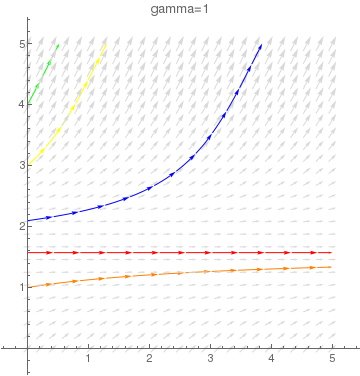
\includegraphics[width=.45\textwidth]{442a}
		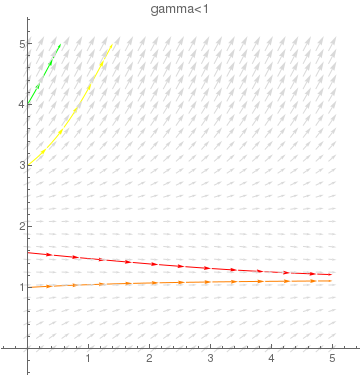
\includegraphics[width=.45\textwidth]{442b}\\
		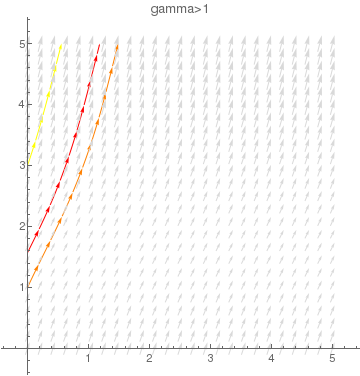
\includegraphics[width=.45\textwidth]{442c}
	\end{center}
	
	If $\theta(0)< \pi/2$ then $\sin(\theta(t)$ increases monotonically from 0 to 1. If $\theta(0)= \pi/2$ (fixed point) then $\sin(\theta(t))=1$. Otherwise $\sin(\theta(t))$ is periodic since the trajectory increases without bound.
	
	If $\gamma < 1$, $\sin(\theta(t))$ is similar to above except the fixed point is now less than $\pi/2$. Lastly, if $\gamma >> 1$ all trajectories increases without bound and $\sin(\theta(t))$ is periodic.
	
	The physical quantity proportional to $\sin(\theta(t))$ is maximum gravitational torque $mgL\sin(\theta)$.
	
	\subsection*{4.4.4}
	\textbf{A.} No, the equation $b\dot{\theta} + mgL\sin\theta = \Gamma - k\theta$ is not a well-defined vector field on the circle, unless $k=0$. For example, even if $\theta = 0 = 2\pi$ is the same space on the circle, $b\dot{\theta}(2\pi) = \Gamma - 2k\pi \neq \Gamma = b\dot{\theta}(0)$.\\
	
	\textbf{B.} Dividing the equation by mgL, we get \\
	$\frac{b\dot{\theta}}{mgL} + \sin\theta = \frac{\Gamma}{mgL} - \frac{k\theta}{mgL}$.\\
	Let $\tau = \frac{mgL}{b}$, $\gamma = \frac{\Gamma}{mgL}$, and $\alpha = \frac{k}{mgL}$.\\
	Then, the above can be expressed as $\theta' = \gamma - \alpha \theta - \sin \theta$, where $\theta' = \frac{d\theta}{d\tau}$.
	
	\textbf{C.} Using values $\gamma=5,\alpha=5/2$, the phase portrait below gives the behavior of $\theta$ from different initial conditions.
	\begin{center}
		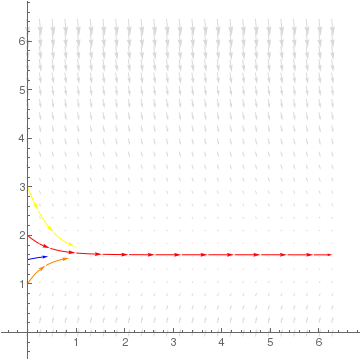
\includegraphics[width=.5\textwidth]{444}
	\end{center}
	It is obvious that only a stable fixed point exists and the pendulum will approach this as $t \to \infty$.
	
	\textbf{D.} For showing the bifurcations, we solve the equations
	\begin{align*}
	\Gamma-k\theta-mgL\sin(\theta)&=0\\
	mgL\cos(\theta)&=-k\\
	\to mgL(\sin(\theta)-\theta\cos(\theta))&=\Gamma
	\end{align*}
	There are many solutions to the last equality, showing that many bifurcation points can occur on different values of $k$. This is made possible by saddle-node bifurcations.
	
	\subsection*{4.5.1 A}
	\begin{figure}[H]
		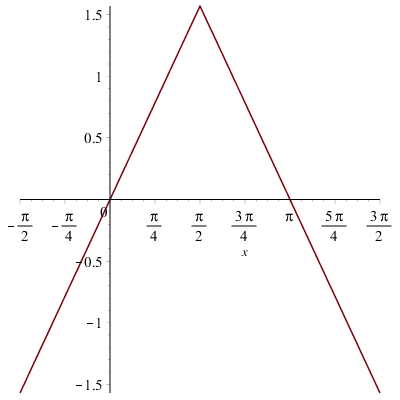
\includegraphics[width=\textwidth]{img/4-5-1a.png}
	\end{figure}
	
	\subsection*{4.5.1 B}
	
	The firefly is able to synchronize the frequency when $\dot \phi = 0$
	
	\begin{equation*}
	\dot \phi =  \dot \Theta - \dot \theta = 0 = \Omega - (\omega + Af(\phi))
	\end{equation*}
	\begin{equation*}
	\Omega = \omega + Af(\phi)
	\end{equation*}
	
	Since $f(\phi) \in [-\pi/2, \pi/2]$, then the range of entrainment should be
	
	\begin{equation*}
	\omega - \frac{A\pi}{2} \leq \Omega \leq \omega + \frac{A\pi}{2}
	\end{equation*}
	\\
	
	\subsection*{4.5.1 C} Assuming that the firefly is phaselocked to the stimulus, $\dot \phi = \Omega - \omega - Af(\phi^*) = 0$.
	
	\begin{align*}
	f(\phi^*) = \frac{\Omega - \omega}{A}
	\end{align*}\\
	
	So as shown in the range of entrainment $|f(\phi^*)| < \frac{\pi}{2}$. 
	
	\subsection*{4.5.1 D}
	\begin{align*}
	T_{drift} &= \int_{-\pi/2}^{\pi/2} \cfrac{d\phi}{\Omega - \omega + A\phi} + \int_{\pi/2}^{3\pi/2} \cfrac{d\phi}{\Omega - \omega + A\pi - A\phi}\\
	& = A\int_{-\pi/2}^{\pi/2} \cfrac{d\phi}{\frac{\Omega - \omega}{A} + \phi} + A\int_{\pi/2}^{3\pi/2} \cfrac{d\phi}{\frac{\Omega - \omega}{A} + \pi - \phi}\\
	& =  \frac{2}{A} ln \Bigg(\frac{\frac{\Omega - \omega}{A} + \frac{\pi}{2}}{\frac{\Omega - \omega}{A} - \frac{\pi}{2}} \Bigg)
	\end{align*}
	
	\subsection*{4.5.3 A}
	As shown in the graph below, there is a single fixed point that attracts all values of $\theta$. The graph also shows that if $\theta$ is beyond the unstable fixed point, then it will undergo a large excursion through $2\pi$ to reach the stable fixed point. Therefore, the rest state is the stable fixed point, while the threshold is the unstable fixed point.\\
	
	\begin{figure}[H]
		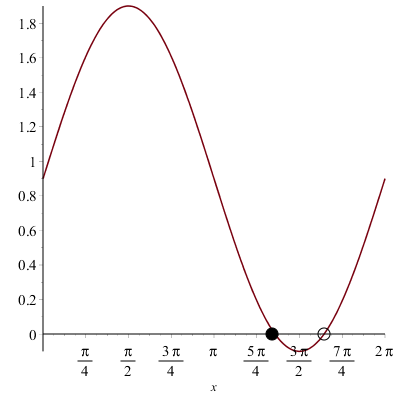
\includegraphics[width=\textwidth]{img/4-5-3a.png}
	\end{figure}
	
	\subsection*{4.5.3 B} The graph of $V(t)$ for various initial conditions. When the initial value is higher than the threshold, then it will go a huge excursion and then goes to the rest state.
	
	\begin{figure}[H]
		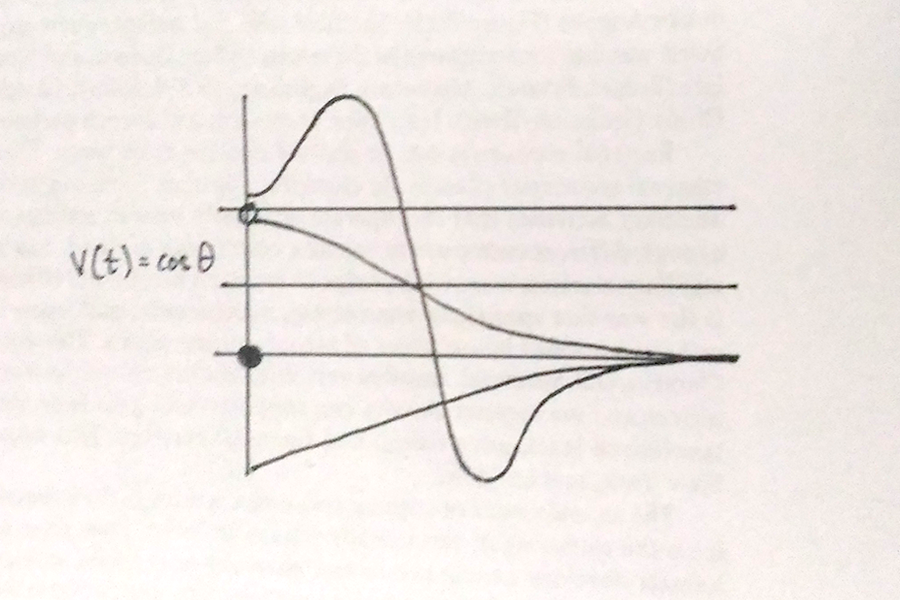
\includegraphics[width=\textwidth]{img/4-5-3b.png}
	\end{figure}
	
	\subsection*{4.6.1}
	\textbf{A.} Using values $I/I_c=1.1,2 \to I_c=10/11,1/2$ we have the following vector fields that shows trajectory of $\phi(t)$ as the vertical coordinate of each point in it. They have same initial condition $\phi(0)=0$.
	
	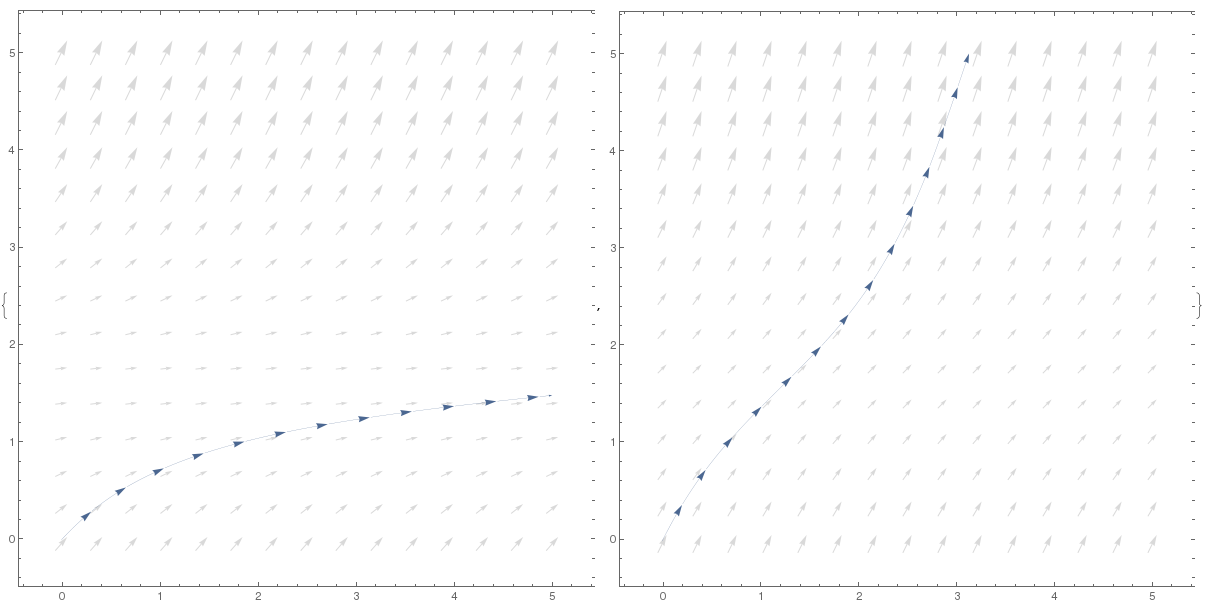
\includegraphics[width=\linewidth]{461a.png}
	
	Observe that for $I/I_c=1.1$ we have $0 < \phi(t) < \pi/2$. Consequently, $0 < \sin\left(\phi(t)\right) < 1$ for a very long time because of the bottleneck exhibited by $\dot{\phi}$. Therefore $0<I_c\sin(\phi(t))<1$, monotonic and aperiodic. For $I/I_c=2$, $\phi(t)$ grows to infinity without bottleneck from $\dot{\phi}$, so $-1 < \sin(\phi(t)) < 1$ and
	$-1/2 < \frac{1}{2}\sin(\phi(t)) < 1/2$ and has a periodic graph.
	
	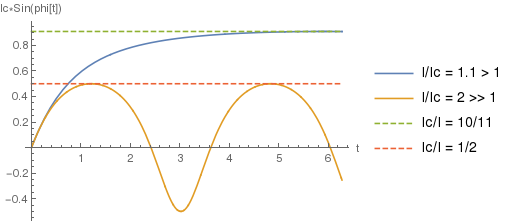
\includegraphics[width=\linewidth]{461b.png}
	
	\textbf{B.} It is given that $V(t)=R-I_cR\sin(\phi(t))$. If $I$ is slightly greater than $I_c$ then $V$ will just go down to 0 from $V=R$. Otherwise, $V$ will just oscillate from $V=R$, as shown from the graph below, where $R=1$.
	
	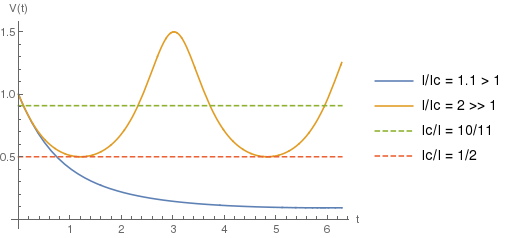
\includegraphics[width=\linewidth]{461c.png}
	
	\subsection*{4.6.2}
	The figures above already shows the graphs $I_x\sin(\phi(t))$ and $V(t)$, solved numerically using Mathematica.
	
	\section*{Chapter 5}
	\subsection*{5.1}
	\textbf{5.1.1} Consider the harmonic oscillator $\dot{x} = v$ , $\dot{v} = - \omega ^2x$.\\
	\textbf{A.} 
	\begin{align*}
	\frac{dx}{dt} \frac{dt}{dv} &= \frac{v}{-\omega^2x}\\
	\frac{dx}{dv} &= \frac{v}{-\omega^2x}\\
	\int -\omega^2xdx &= \int vdv \\
	-\frac{1}{2} \omega^2x^2 &= \frac{1}{2}v^2 + C\\
	\frac{1}{2}v^2 + \frac{1}{2} \omega^2x^2 &= C\\
	\omega^2x^2 + v^2&= C
	\end{align*}
	Since $\omega^2x^2, v^2 \geq 0, C \geq 0$.\\
	\textbf{B.} 
	Multiplying the previous ellipses by $\frac{1}{2}m$
	\begin{align*}
	\frac{1}{2}m\omega^2x^2 + \frac{1}{2}mv^2&= C
	\end{align*}
	Substituting $\omega^2 = \frac{k}{m}$, and taking $C = 0$,
	\begin{align*}
	\frac{1}{2}kx^2 + \frac{1}{2}mv^2&= 0.
	\end{align*}\\
	
	\textbf{5.1.4}\\
	
	$\left[ \begin{array}{c} \dot{x} \\ \dot{y} \end{array} \right] = \begin{bmatrix} 3 & -2 \\ -1 & 2 \end{bmatrix} \left[ \begin{array}{c} x \\ y \end{array} \right]$\\
	
	\textbf{5.1.8}\\
	
	Given $\dot{x} = -2y$ and $\dot{y}=x$. 
	\begin{align*}
	\frac{dx}{dt} \frac{dt}{dy} &= \frac{-2y}{x}\\
	\int xdx &= \int -2ydy \\
	\frac{1}{2}x^2 + y^2 = C.
	\end{align*}
	\\Below is a sketch of typical trajectories. \\
	%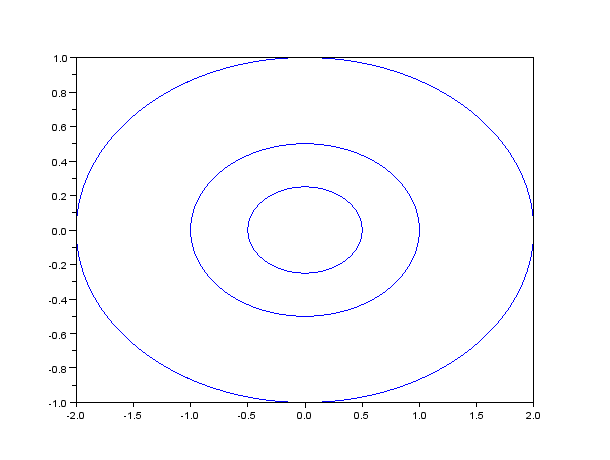
\includegraphics[width=\textwidth]{518.png}
	
	\textbf{5.1.10}\\
	\textbf{A.} $\dot{x}=y$ , $\dot{y}=-4x$. Liapunov. \\
	The phase portrait shows concentric ellipses. While the origin does not attract, trajectories remain close.\\
	
	\textbf{B.} $\dot{x}=2y$ , $\dot{y}=x$. None. \\
	The phase portrait show that the origin repels trajectories.They seem to approach $\pm \infty$ instead.\\
	
	\textbf{C.} $\dot{x}=0$ , $\dot{y}=x$. None. \\
	The phase portrait shows vertical lines that go to $+ \infty$ at the right of the y-axis and go to $ - \infty$ at the left. At $x=0$, there is no line, thus the origin is neither attracting nor Liapunov.\\
	
	\textbf{D.} $\dot{x}=0$ , $\dot{y}=-y$. Liapunov. \\
	The phase portrait shows vertical lines that converge to the x-axis. While the origin is not attracting, it is Liapunov since close trajectories remain close to it.\\
	
	\textbf{E.} $\dot{x}=-x$ , $\dot{y}=-5y$. Asymptotically stable. \\
	The phase portrait shows that the origin is both an attracting and Liapunov fixed point.\\
	
	\textbf{F.} $\dot{x}=x$ , $\dot{y}=y$. None. \\
	The phase portrait shows that the origin a repelling fixed point. It is neither attracting nor Liapunov.
	
	\subsection*{5.2.2 A}
	$\dot x = x - y$\\
	$\dot y = x + y$\\
	
	\begin{math}
	A =  
	\begin{bmatrix}
	1 & -1 \\
	1 & 1
	\end{bmatrix}
	\end{math}
	
	This produces $\Delta = 2$, and $\tau = 2$. Therefore, $\lambda^2 - 2\lambda + 2 = 0$.\\
	Using the quadratic formula,
	\begin{align*}
	\lambda &= \frac{2 \pm \sqrt{4 - 4(2)}}{2}\\
	&= 1 \pm i
	\end{align*}
	
	
	at $\lambda_1 = 1 + i$:
	\begin{math}
	\begin{bmatrix}
	-i & -1 \\
	1 & -i
	\end{bmatrix}
	v_1 =
	\begin{bmatrix}
	0\\
	0
	\end{bmatrix}
	\end{math}\\
	we get $v_1 = (i, 1)$
	\\
	
	at $\lambda_1 = 1 - i$: 
	\begin{math}
	\begin{bmatrix}
	i & -1 \\
	1 & i
	\end{bmatrix}
	v_2 =
	\begin{bmatrix}
	0\\
	0
	\end{bmatrix}
	\end{math}\\
	we get $v_2 = (-i, 1)$\\
	
	\subsection*{5.2.2 B}
	let $e^{i\omega t} = cos \omega t + i sin \omega t$\\
	\begin{align*}
	x(t) &= C_1 e^{(1 + i)t}v_1 + C_2 e^{(1 - i)t}v_2\\
	& = \begin{bmatrix}
	C_1 e^t i cos (t) - C_1 e^t sin (t) - C_2 e^t i cos (t) - C_2 e^t sin (t) \\
	C_1 e^t cos (t) + C_1 e^t i sin (t) + C_2 e^t cos (t) - C_2 e^t i sin (t)
	\end{bmatrix}\\
	& = i e^t (C_1 - C_2)
	\begin{bmatrix}
	cos (t) \\
	sin (t)
	\end{bmatrix}
	+ e^t (C_1 + C_2)
	\begin{bmatrix}
	-sin (t)\\
	cos (t)
	\end{bmatrix}
	\end{align*}\\
	
	\subsection*{5.2.4}
	\begin{align*}
	\dot x &= 5x + 10y\\
	\dot y &= -x - y
	\end{align*}\\
	The eigenvectors are not real since the eigenvalues are $\lambda = 2 \pm i$. The fixed point at $(0,0)$ is an unstable spiral since $\tau > 0$.
	
	\begin{figure}[H]
		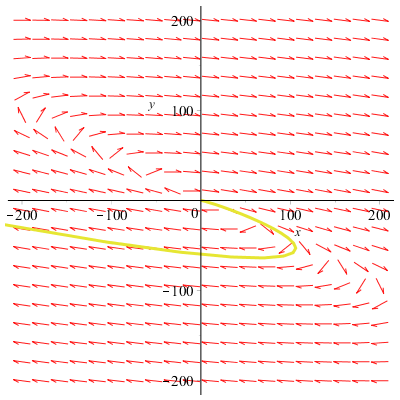
\includegraphics[width=\textwidth]{img/5-2-4.png}
	\end{figure}
	
	\subsection*{5.2.12 A}
	let $x = I$ and $y = \dot I$
	
	\begin{align*}
	0 & =L \dot y + Ry + \frac{x}{C} \\
	\dot y & = \frac{-Ry}{L} - \frac{x}{CL}
	\end{align*}\\
	
	So the 2-dimensional linear system is given by:
	
	\begin{align*}
	\dot x &= y\\
	\dot y & = \frac{-Ry}{L} - \frac{x}{CL}
	\end{align*}\\
	
	\subsection*{5.2.12 B}
	\begin{equation}
	\begin{split}
	\Delta & = \frac{1}{CL} \\
	\tau & = -\frac{R}{L} \\
	\lambda_{1,2} &= \frac{\tau \pm \sqrt{\tau^2 - 4\Delta}}{2}
	\end{split}
	\end{equation}\\
	
	If $R > 0$, then $\lambda_1$ and $\lambda_2$ are both negative. It is both attracting and Liapunov stable. Therefore, it is asymptotically stable. If $R = 0$, the eigenvalues are purely imaginary since $\Delta > 0$ and $\tau = 0$. This means that we have a neutrally stable center.
	
	\subsection*{5.2.12 C}
	When $R^2C-4L > 0$, we have stable node since eigenvalues are negative real numbers.
	
	\begin{figure}[H]
		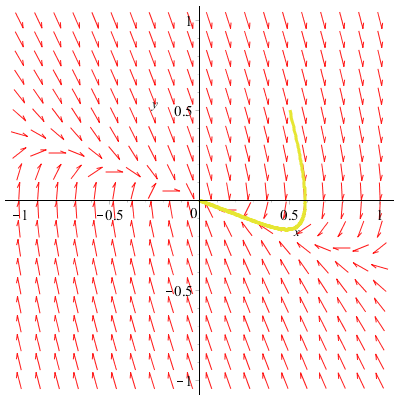
\includegraphics[width=\textwidth]{img/5-12-3p.png}
	\end{figure}
	
	When $R^2C-4L < 0$, the real part of the eivenvalues are negative but the imaginary part is not zero so we have a stable spiral.
	
	\begin{figure}[H]
		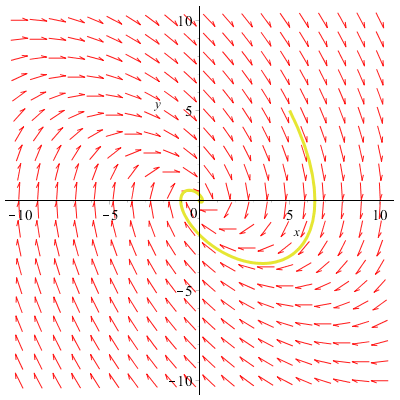
\includegraphics[width=\textwidth]{img/5-12-3n.png}
	\end{figure}
	
	
	When $R^2C-4L = 0$, we have a degenerate node.
	
	\begin{figure}[H]
		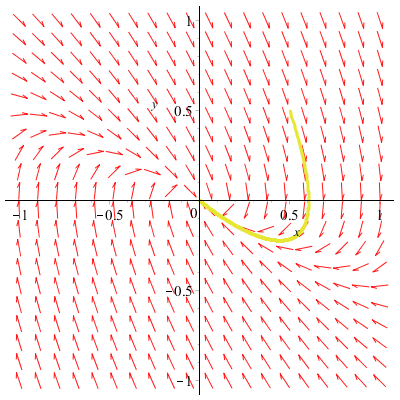
\includegraphics[width=\textwidth]{img/5-12-3z.png}
	\end{figure}
	
	
	\subsection*{5.2.14}
	If $a, b, c, d \in [-1,1]$, then the maximum determinant $\Delta = 2$ and the maximum trace $\tau = 2$. Using the Monte Carlo Method, we have the following plot:
	
	\begin{figure}[H]
		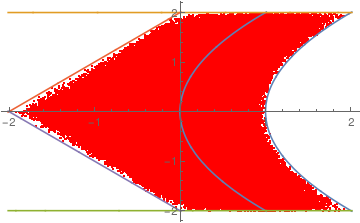
\includegraphics[width=\textwidth]{img/5-2-14a.png}
	\end{figure}
	
	We assume that the bounds at the right is $\Delta = \tau^2 +1$ and the bounds at the left is $\Delta = \tau + 2$ for $\tau < 0$ and $\Delta = \tau - 2$ for $\tau > 0$ as shown above.
	
	We now find the area.
	
	\begin{align*}
	2 \int_0^2 [\tau + 1 - (\tau - 2)] d\tau &= 2(\frac{20}{3})
	\end{align*}
	
	Recall that in the figure 5.3.8 of Nonlinear Dynamics and Chaos (Strogatz), the distribution of different types of fixed points was shown in a graph.\\
	
	Now to get the probabilities of the saddle point, we find the area of the region where $\Delta < 0$. By observation, the area is equal to 4. We divide it by the total area so $\frac{4}{40/3} = \frac{3}{10} = 30\%$.\\
	
	We use the same approach to find the probability of the stable and unstable nodes. $\int_0^2 \frac{\tau^2}{4} d\tau = \frac{2}{3}$. The probability for the stable and unstable nodes are both $\frac{2/3}{40/3} = 5\%$.\\
	
	The probability for spirals is $1 - P(others) = 1 - (0.3 + 2(0.5)) = 0.6$. Then the probability for a stable and usntable spliral is $\frac{0.6}{2} = 30\%$. The probabilities of non-isolated fixed points, degenerate nodes, stars, and centers are practically 0.\\
	
	If we use a a normal distribution, the answer is not the same as shown in the plot given by the Monte Carlo Method.
	\begin{figure}[H]
		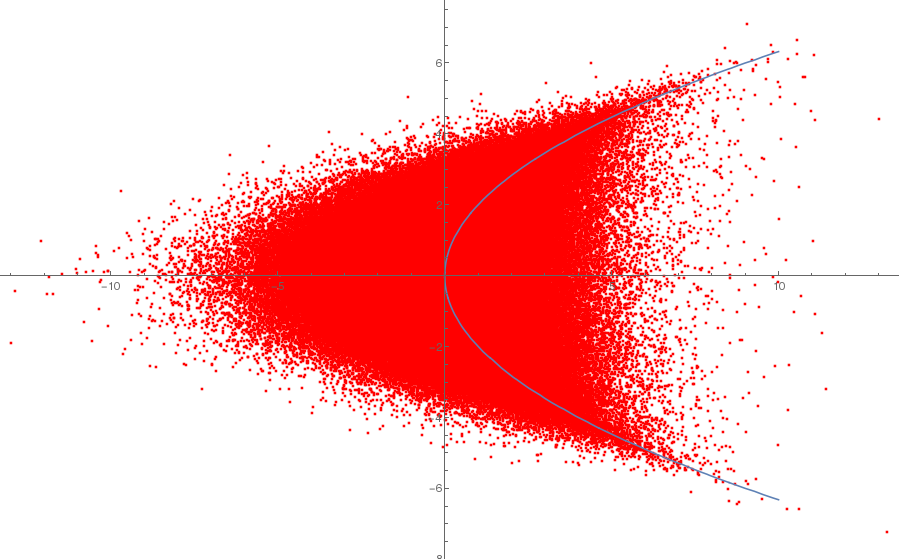
\includegraphics[width=\textwidth]{img/5-2-14b.png}
	\end{figure}
	
	
	\subsection*{5.3.2}
	\textbf{A}. Romeo's love for Juliet depends solely on her love for him and not vice-versa. This suggests that if she loves him, she should express her feelings to him. Juliet's love for Romeo depends on her love for him but diminishes by the rate of his love for her.
	
	\textbf{B.} If both have no feelings for each other $R=J=0$, nothing will happen. Given the phase portrait below, the origin is unstable. If the initial condition is perturbed, it will result to love/hate relationship that always changes and goes in circular motion.
	\begin{figure*}[h!]
		\centering
		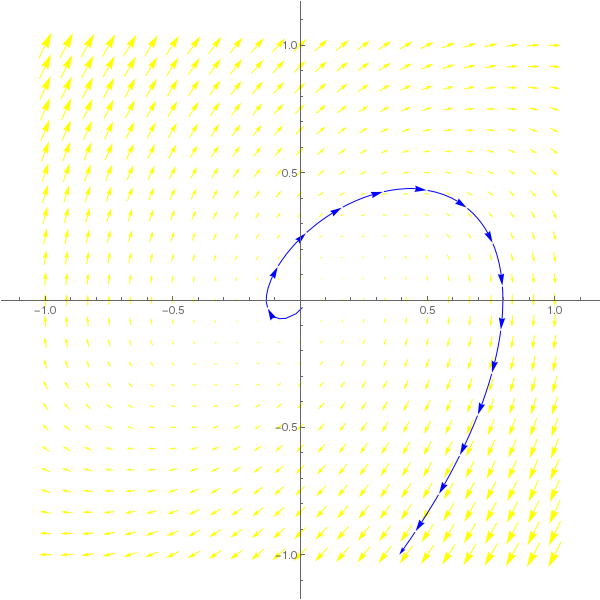
\includegraphics[width=.6\textwidth]{532a.png}
	\end{figure*}
	
	\textbf{C.} The solution of system using initial conditions $R(0)=1,J(0)=0$ is given by
	\begin{align*}
	R(t) &= -\frac{2}{3}\mathbf{e}^{\frac{t}{2}}\sin\left(\frac{\sqrt{3}}{2}t\right)\\
	J(t) &=
	\frac{1}{3}\mathbf{e}^{t/2}\left[3\cos\left(\frac{\sqrt{3}}{2}t\right)-\sqrt{3}\sin\left(\frac{\sqrt{3}}{2}t\right)\right]
	\end{align*}
	
	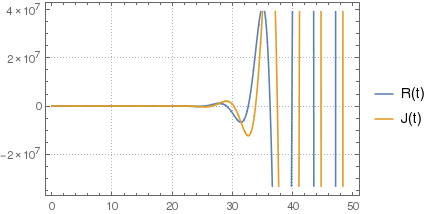
\includegraphics[width=\textwidth]{532b.png}
	
	\subsection*{5.3.4} Let $\dot{R} = aR +bJ,$ and $\dot{J} = -bR - aJ$ so the fixed point is at $(0,0)$. The trace of matrix is $\tau=0$, while the determinant is $\Delta=b^2-a^2$. The plot of $\text{sgn}(\Delta)$ on $(a,b)$ plane is given below.
	
	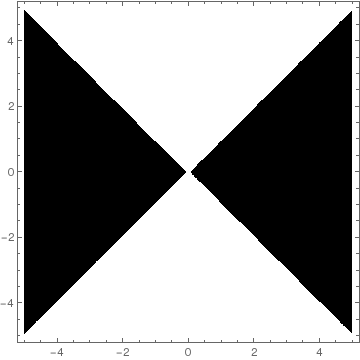
\includegraphics[width=.5\textwidth]{534a.png}
	
	White regions are the collection of points that $\Delta>0$, black regions represent $\Delta<0$ and the "X" curve makes $\Delta=0$. If $\Delta>0$ we have a stable isolated center that comprises of ellipses. Next, if $\Delta=0$ we have a plane of nonisolated fixed points and if $\Delta<0$ we have a saddle isolated fixed point.
	
	
	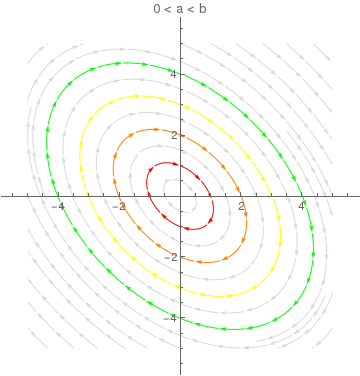
\includegraphics[width=.45\textwidth]{534b1.png}
	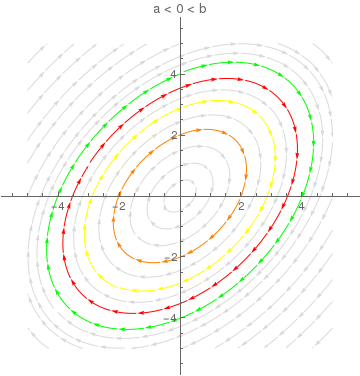
\includegraphics[width=.45\textwidth]{534b2.png}
	
	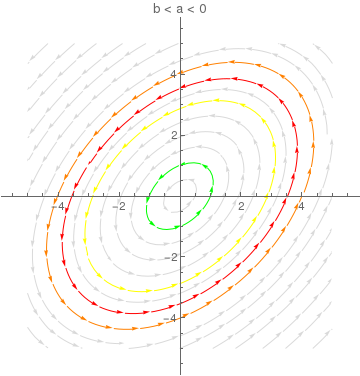
\includegraphics[width=.45\textwidth]{534b3.png}
	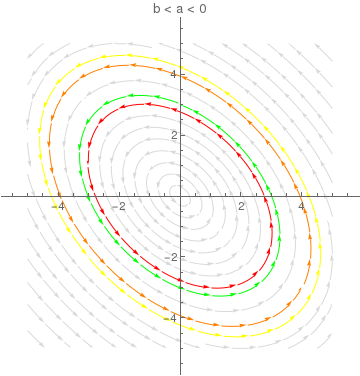
\includegraphics[width=.45\textwidth]{534b4.png}
	
	
	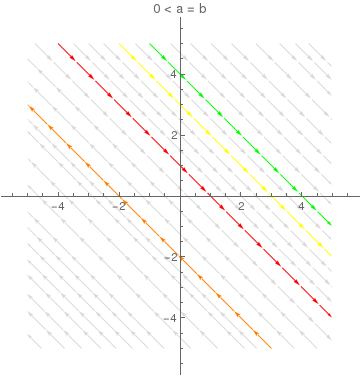
\includegraphics[width=.45\textwidth]{534c1.png}
	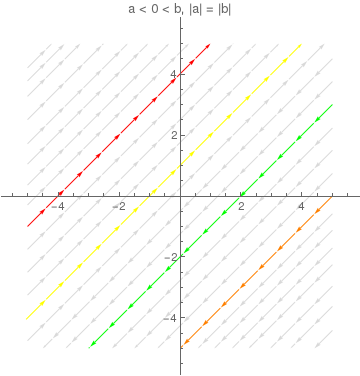
\includegraphics[width=.45\textwidth]{534c2.png}
	
	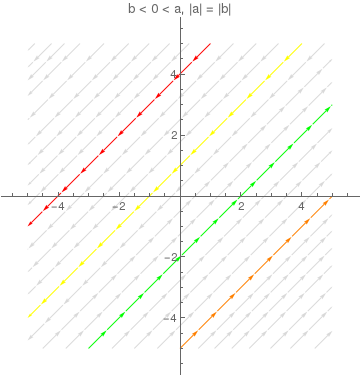
\includegraphics[width=.45\textwidth]{534c3.png}
	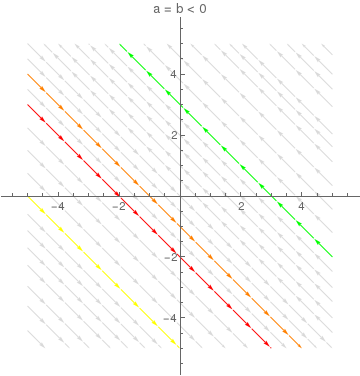
\includegraphics[width=.45\textwidth]{534c4.png}
	
	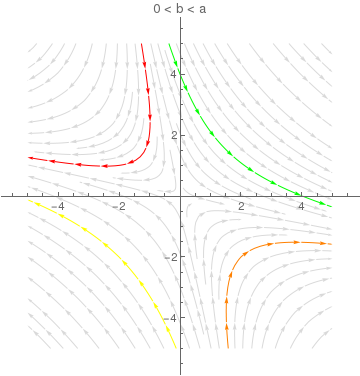
\includegraphics[width=.45\textwidth]{534d1.png}
	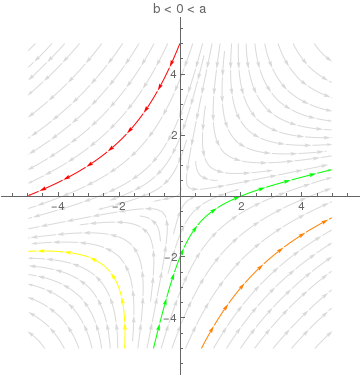
\includegraphics[width=.45\textwidth]{534d2.png}
	
	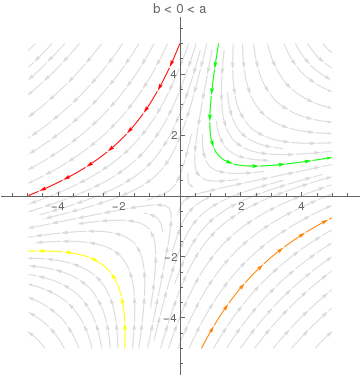
\includegraphics[width=.45\textwidth]{534d3.png}
	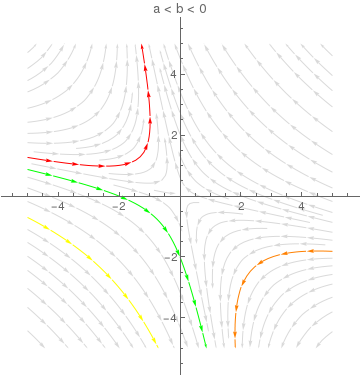
\includegraphics[width=.45\textwidth]{534d4.png}
	
	\subsection*{5.3.6} Trace is $\tau=b$ and determinant is $\Delta=0$ and we have a line of Lyapunov stable fixed points. Analyzing the vector fields in varying signs of $a$ and $b$, we have the following:
	
	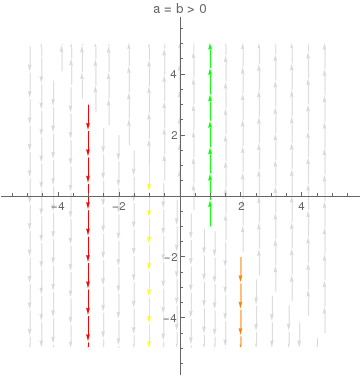
\includegraphics[width=.45\textwidth]{536a.png}
	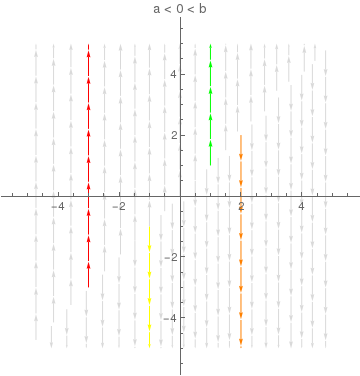
\includegraphics[width=.45\textwidth]{536b.png}
	
	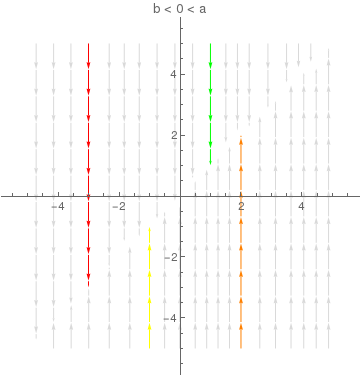
\includegraphics[width=.45\textwidth]{536c.png}
	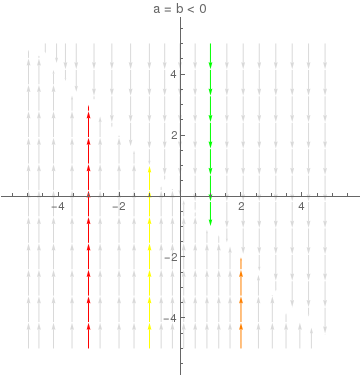
\includegraphics[width=.45\textwidth]{536d.png}
	
	Juliet's feelings depend on $a$,$b$ and specified initial condition. For example, if $a,b>0$ and $R(0),J(0)>0$, Juliet ends up loving him.
	
	\section*{Chapter 6}
	\subsection*{6.1}
	\textbf{6.1.2}\\
	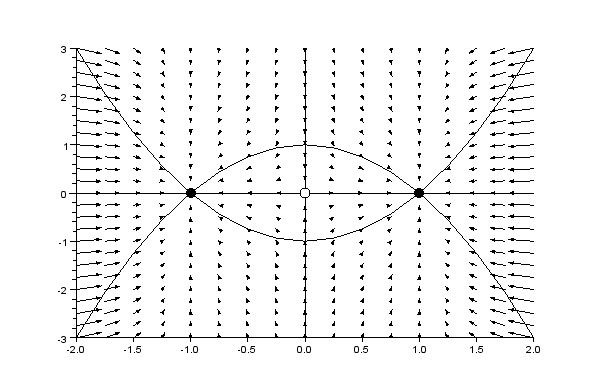
\includegraphics[width=\textwidth]{612n.png}
	
	\subsection*{6.2.1}
	No. Aside from the intersection points, but we should also look at the direction of these trajectories. They might "intersect" at fixed points, but the trajectories will just stop at the intersection because fixed points may be sinks.
	\subsection*{6.2.2}
	Consider the system $\dot{x} = y$, $\dot{y} = -x + (1 - x^2 - y^2)y$. \\
	\textbf{A.} Let D be the open disk $x^2 + y^2 < 4$. Let \textbf{f(x)} = $ \begin{bmatrix}
	y \\
	-x + (1 - x^2 - y^2)y
	\end{bmatrix}.$ 
	\\Both components are continuous since they are polynomials. Now, taking the partial derivatives with respect to $x$ and $y$, we get \\
	\textbf{$\frac{\partial f}{\partial x}$} = $\begin{bmatrix}
	0 \\
	-1 -2xy
	\end{bmatrix}$ and \textbf{$\frac{\partial f}{\partial y}$} = $\begin{bmatrix}
	1 \\
	1 - x^2 - 3y^2
	\end{bmatrix}$, \\ 
	where each component is also continuous since each is a polynomial. Thus, the existence and uniqueness theorem applies in the disk D. \\
	
	\textbf{B.} Let $x(t) = \sin t$ and $y(t) = \cos t$. Then, \begin{align*}
	\dot{x} &= y(t) = \cos t = \dot{x}\\
	\dot{y} &= -x + (1 - x^2 - y^2)y \\
	&= - \sin t + (1 - \sin^2 t - \cos^2 t)\cos t \\
	&= - \sin t + (1 - 1)\cos t \\
	&= - \sin t \\
	&= \dot{y}.
	\end{align*}
	
	\textbf{C.} Consider a different solution starting from the initial condition 
	$x(0) = \frac{1}{2}$, $y(0) = 0$. It is clear that this initial solution is inside the disk D from (a). Thus, within D, trajectories do not intersect. From (b), it can be seen that the trajectory $x^2 + y^2 = 1$ is a solution. Since the given solution starts from inside this circle, and will not intersect it, the solution satisfies $x(t)^2 + y(t)^2 < 1$,  $\forall t < \infty$ .
	
	\subsection*{6.3.6}
	\begin{align*}
	\dot x &= xy - 1  \\
	\dot y &= x - y^3
	\end{align*}
	
	\begin{equation*}
	A =
	\begin{bmatrix}
	y & x \\
	1 & -3y^2
	\end{bmatrix}
	\end{equation*}
	
	Fixed points are (1, 1) and (-1, -1).\\
	
	at (1, 1):
	\begin{equation*}
	\begin{bmatrix}
	1 & 1 \\
	1 & -3
	\end{bmatrix}    
	\end{equation*}
	
	The eigenvalues are $\lambda_{1, 2} = -1 \pm \sqrt{5}$, so this is a saddle point since $\Delta = \lambda_1 \lambda_2 = -4$. The unstable manifold goes out at the direction of $v_1 = (2+\sqrt{5}, 1)$.\\
	
	at (-1, -1):
	\begin{equation*}
	\begin{bmatrix}
	-1 & -1 \\
	1 & -3
	\end{bmatrix}    
	\end{equation*}
	
	
	The eigenvalue is $\lambda = -2$, so this is a degenerate node since $\Delta = 4$, and $\tau = -4$.\\
	
	\begin{figure}[H]
		\centering
		\subfloat[nullclines]
		{{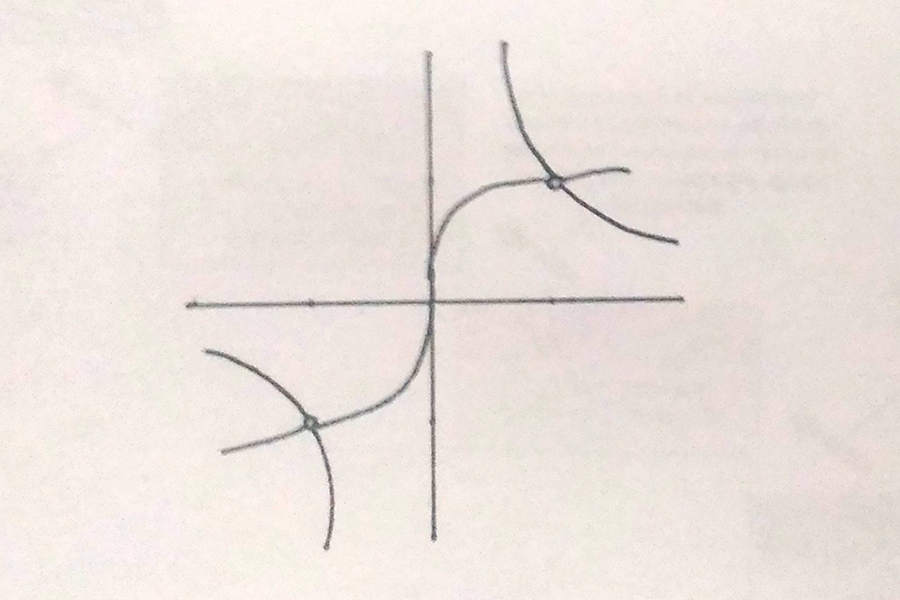
\includegraphics[width=5cm]{img/6-3-6a.png} }}%
		\qquad
		\subfloat[phase portrait]
		{{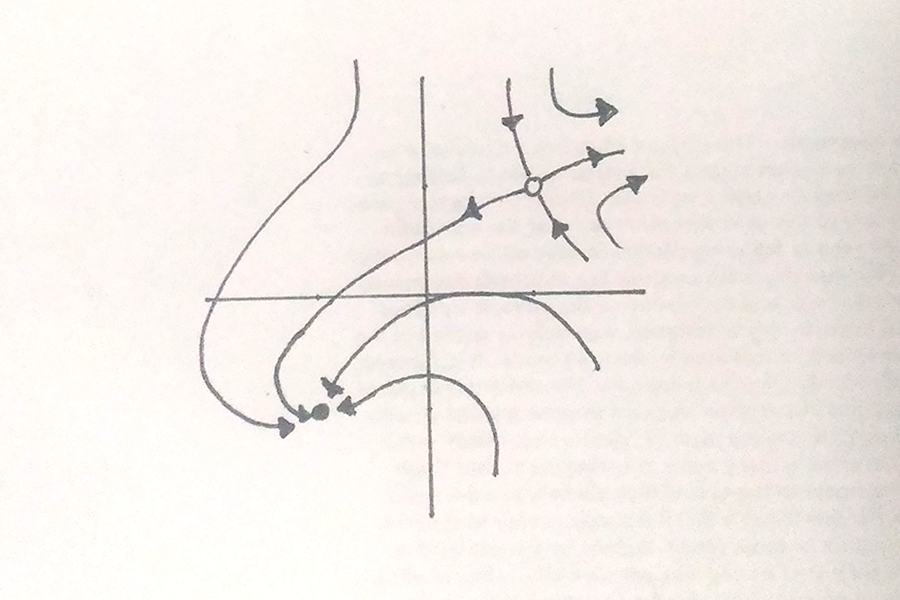
\includegraphics[width=5cm]{img/6-3-6b.png} }}%
		\qquad
		\caption{}%
		\label{fig:example}%
	\end{figure}
	
	\subsection*{6.3.10}
	Let $\dot{x}=xy$ and $\dot{y}=x^2-y$, then the Jacobian is $A=\begin{pmatrix}
	y & x \\
	2x & -1
	\end{pmatrix}$ and $A(0,0) = \begin{pmatrix}
	0&0\\
	0&-1
	\end{pmatrix}$. The trace is $\tau=y-1$, $\tau(0,0)=-1$ and determinant is $\Delta=-y-2x^2$, $\Delta(0,0)=0$.
	
	\textbf{A.} By linearization, the system has non-isolated Lyapunov stable fixed points since $\Delta(0,0)=0$ and $\tau(0,0)<0$.
	
	\textbf{B.} Considering the global $\Delta=-(y+2x^2)$, it can be greater or less than zero in the neighborhood of origin. Therefore it is an isolated fixed point.
	
	\textbf{C.} The analysis of nullclines are given below:
	
	
	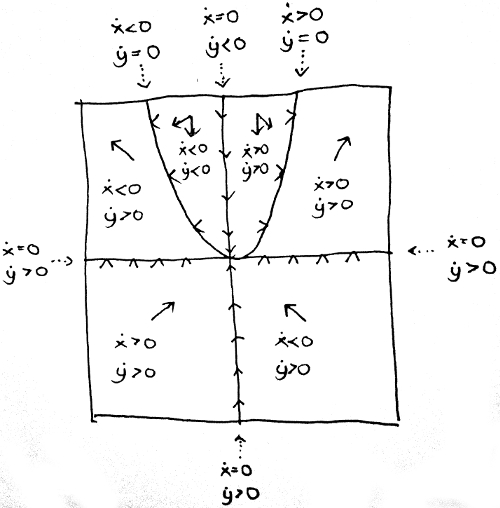
\includegraphics[width=.5\textwidth]{6310c}
	
	\textbf{D.} The phase portrait with nullclines is generated by Mathematica below together with some trajectories.
	
	
	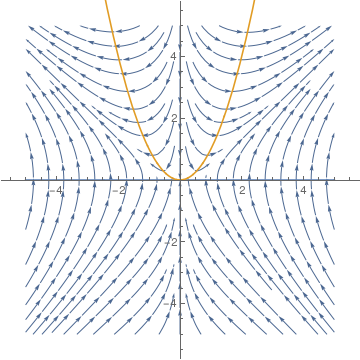
\includegraphics[width=.45\textwidth]{6310a.png}
	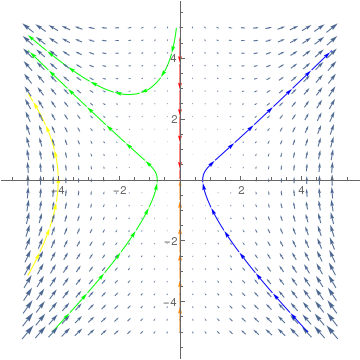
\includegraphics[width=.45\textwidth]{6310b.png}
	
	\subsection*{6.4.2}
	Consider $\dot{x} = x(3 - 2x - y)$ and $\dot{y} = y(2 - x- y)$.\\
	The fixed points are $(0,0)$ , $(1,1)$, $(0,2)$, $(\frac{3}{2},0)$.\\
	The Jacobian is $A = \begin{bmatrix}
	3 - 4x - y & -x \\
	-y & 2 - x - 2y
	\end{bmatrix}$. Checking the stability of the fixed points, \begin{align*}
	A(0,0) &= \begin{bmatrix}
	3 & 0 \\
	0 & 2
	\end{bmatrix} & , & &\lambda &= 3,2 &\quad \\
	A(1,1) &= \begin{bmatrix}
	-2 & -1 \\
	-1 & -1
	\end{bmatrix} & , & &\lambda &= \frac{-3 \pm \sqrt{5}}{2} &\quad \\
	A(0,2) &= \begin{bmatrix}
	1 & 0 \\
	-2 & -2
	\end{bmatrix} & , &&\lambda &= 1,-2 &\quad \\
	A(\frac{3}{2},0) &= \begin{bmatrix}
	-3 & -\frac{3}{2} \\
	0 & \frac{1}{2}
	\end{bmatrix} & , &&\lambda &= -3,\frac{1}{2} &\quad\\
	\end{align*}
	where $\lambda$ are the eigenvalues of each matrix.\\ 
	Thus, (0,0) is a repeller, (1,1) is an attractor, and (0,2) and ($\frac{3}{2}$,0) are saddle points. The plot below shows the nullclines. It can be seen that the basin of attraction is $x, y > 0$.
	
	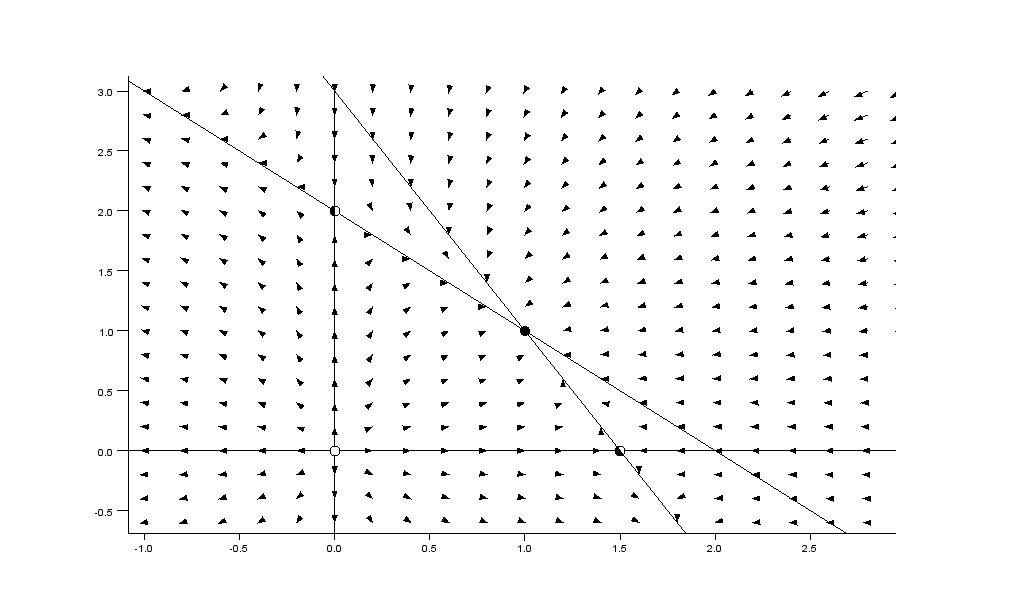
\includegraphics[width=\textwidth]{642.png}
	
	
	
	\subsection*{6.4.7 A}
	Let $x = n_1$ and $y = n2$.
	\begin{align*}
	\dot x = G_1 N_0 x - G_1 \alpha_1 x^2 - G_1 \alpha_1 xy - k_1 x\\
	\dot x = G_2 N_0 y - G_2 \alpha_2 y^2 - G_2 \alpha_2 xy - k_2 y\\
	\end{align*}
	
	The Jacobian matrix at $(0, 0)$ of is given by
	
	\begin{equation*}
	\begin{bmatrix}
	G_1 N_0 - k_1 & 0\\
	0 & G_2 N_0 - k_2
	\end{bmatrix}
	\end{equation*}
	
	$\tau = (G_1 + G_2)N_0 - (k_1+k_2)$ and $\Delta = (G_1 N_0 - k_1)(G_2 N_0 - k_2)$. This means that the fixed point at $(0,0)$ is unstable when $(G_1 + G_2)N_0 > (k_1+k_2)$ and stable when $(G_1 + G_2)N_0 < (k_1+k_2)$.\\
	
	Let $a = G_1 N_0 - k_1$ and $b = G_2 N_0 - k_2$. This yields $\tau = a + b$ and $\Delta = ab$. It is a saddle point when one of a or b is negative; that is $k_1 > G_1 N_0$ xor $k_2 > G_2 N_0$.
	
	\begin{align*} 
	\tau^2 - 4 \Delta &= (a + b)^2 - 4ab\\
	&= a^2 + b^2 - 2ab\\
	&= (a-b)^2
	\end{align*} 
	
	It is always positive. Therefore those fixed points are not saddle points are either stable or unstable nodes.
	
	\subsection*{6.4.7 B}
	The other fixed points that may exist are
	
	\begin{equation*}
	\Bigg( \frac{k_1 - G_1 N_0}{G_1 \alpha_1}, 0 \Bigg),
	\Bigg( 0, \frac{k_2 - G_2 N_0}{G_2 \alpha_2} \Bigg),
	\Bigg( \frac{G_1 k_2 - G_2 k_1}{G_1 \alpha_1 (G_1 - G_2)}, \frac{G_1 N_0 - G_2 N_0 - k_1 + k_2}{\alpha_2 (G_1 - G_2)} \Bigg)
	\end{equation*}
	
	\subsection*{6.4.7 C}
	
	Any closed orbit in the phase plane must enclose fixed points whose indices sum up to $+1$. There can only be 3 or 1 fixed points. If there are 3 fixed points, then there should also be 3 qualitatively different phase portraits since there can only be one saddle point at a time and any combination of stable and unstable fixed point. If there is one fixed point, then there can be 2 (stable and unstable). Therefore there are 5 qualitatively different phase portrait. This also says that the laser will eventually turn into a lamp when there are more unstable fixed points in the phase plane.
	
	\subsection*{6.5.10} Let $\ddot{u}+u=\alpha+\epsilon u^2$.
	
	\textbf{A.} The system can also be written as $\dot{u}=v$ and $\dot{v}=\alpha+\epsilon u^2-u$.
	
	\textbf{B.} The equilibrium points in $(u,v)$ are given by $\left(\frac{1\pm\sqrt{1-4\epsilon\alpha}}{2\epsilon},0\right)$.
	
	\textbf{C.} For this system, the Jacobian is $A=\begin{pmatrix}
	0&1\\
	2\epsilon u-1 & 0
	\end{pmatrix}$, trace $\tau=0$ and determinant $\Delta=1-2\epsilon u$. For a fixed point to be a center, it must satisfy $\Delta>0$ and $\tau=0$.
	\begin{align*}
	1-2\epsilon u &> 0\\
	2\epsilon u &< 1\\
	u &< \frac{1}{2\epsilon}
	\end{align*}
	Clearly, the fixed point $u_c=\left(\frac{1-\sqrt{1-4\epsilon\alpha}}{2\epsilon},0\right)$ satisfies the condition above and is indeed the center since $\Delta=\sqrt{1-4 a e}>0$. Note that the other fixed point is a saddle, since it makes $\Delta=-\sqrt{1-4 a e}<0$.
	
	If it is a nonlinear center, then all trajectories must orbit this point. But  there exists another fixed point that is a saddle, therefore $u_c$ is not a nonlinear center.
	
	\textbf{D.} On part C above, we showed that $u_c$ is a local center and thus can correspond to a circular planetary orbit where $(u,v)$ is the displacement of a planet. A realization of this trajectory is shown below with values $\alpha=1$, $\epsilon=0.001$ and initial displacement $(10,0)$. The next figure shows that $u_c$ is not a nonlinear center as shown by two trajectories that include $(300,300)$ and $(700,700)$.
	
	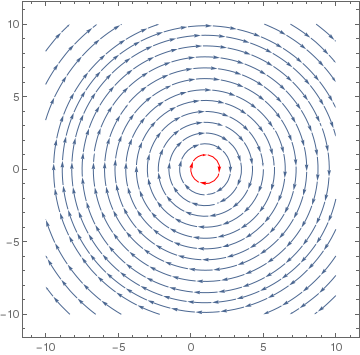
\includegraphics[width=.45\textwidth]{6510.png}
	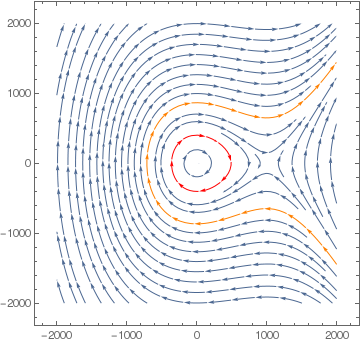
\includegraphics[width=.47\textwidth]{6510b.png}
	
	\subsection*{6.5.14}
	Consider a glider flying at speed $v$ at an angle $\theta$ to the horizontal with motion governed by the equations $\dot{v} = -\sin \theta - Dv^2$ and $v\theta = -\cos \theta + v^2$, \\
	\textbf{A.} Suppose there is no drag (D=0). To show that $E(v,\theta) = v^3 - 3v\cos \theta$ is conservative, it is enough to show that $\frac{dE}{dt} = 0$.\\
	\begin{align*}
	\frac{dE}{dt} &= 3v^2\dot{v} - 3\cos \theta \dot{v} + 3v\sin \theta \dot{\theta}\\
	&= 3v^2 (-\sin \theta - Dv^2) - 3 \cos \theta (- \sin \theta - Dv^2) + 3\sin \theta (- \cos \theta + v^2)\\
	&= -3v^2\sin \theta + 3 \cos \theta \sin \theta - 3 \cos \theta \sin \theta + 3v^2\sin \theta , since D=0\\
	&=0. 
	\end{align*}\\
	Thus E is conservative. The phase portrait is shown below with fixed points at $(v,\theta) = (\pm 1, 0)$. It shows that if the glider starts at $(\pm 1,0)$, it is stable. \\ 
	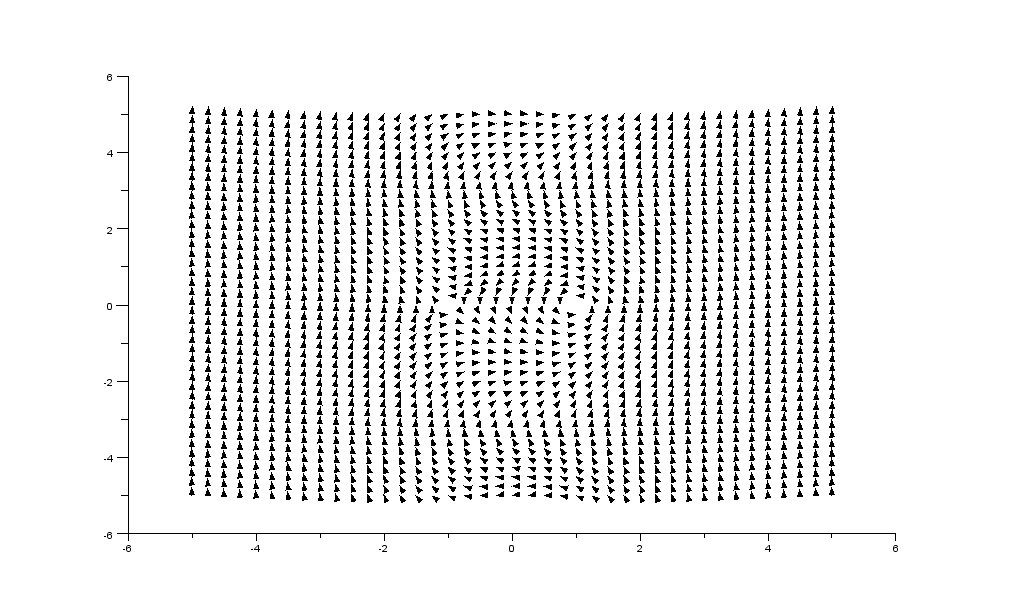
\includegraphics[width=\textwidth]{6514.png}
	\\
	\textbf{B.} Suppose $D > 0$. The new fixed points are at $(v,\theta) = (\pm \sqrt{\cos(\arctan(-D)}, \arctan(-D))$. From the plot below at D=1, it can be seen that they are attracting fixed points. Thus, this system is not conservative.\\  
	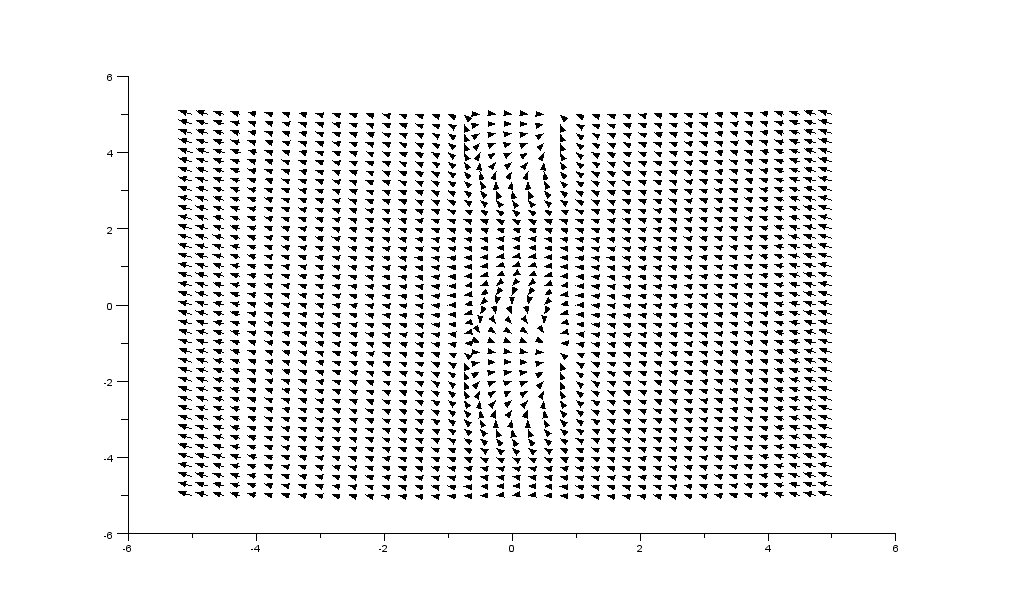
\includegraphics[width=\textwidth]{65142.png}
	
	\subsection*{6.6.6 A} The nullclines of $\dot x = 0$ and $\dot y = 0$
	\begin{figure}[H]
		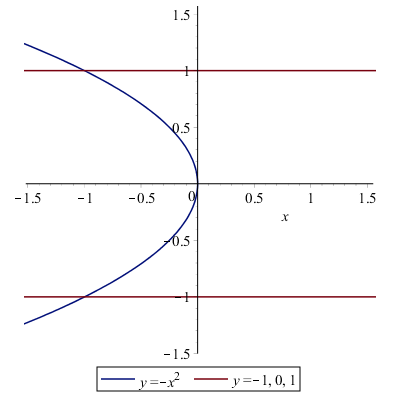
\includegraphics[width=\textwidth]{img/6-6-6a.png}
	\end{figure}
	
	\subsection*{6.6.6 B} The signs of $\dot x$ and $\dot y$ in different regions
	\begin{figure}[H]
		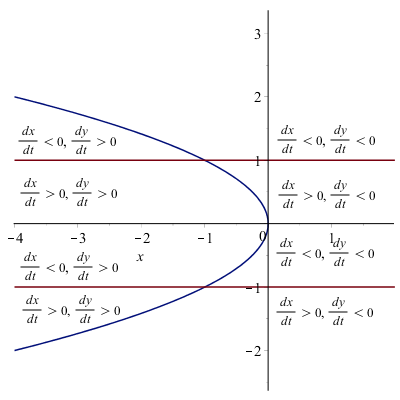
\includegraphics[width=\textwidth]{img/6-6-6b.png}
	\end{figure}
	
	\subsection*{6.6.6 C} The Jacobian matrix is
	
	\begin{equation*}
	\begin{bmatrix}
	0 & 1-3y^2 \\
	-1 & -2y
	\end{bmatrix}
	\end{equation*}
	
	At (-1, 1):
	\begin{equation*}
	\begin{bmatrix}
	0 & -2\\
	-1 & -2
	\end{bmatrix}
	\end{equation*}
	
	The eigenvalues are $\lambda_{1,2} = -1 \pm \sqrt{3}$. The eigenvectors are $v_1 = (-1-\sqrt{3}, 1)$ and $v_2 = (-1+\sqrt{3}, 1)$.\\
	
	At (-1, -1):
	\begin{equation*}
	\begin{bmatrix}
	0 & -2\\
	-1 & 2
	\end{bmatrix}
	\end{equation*}
	
	The eigenvalues are $\lambda_{1,2} = 1 \pm \sqrt{3}$. The eigenvectors are $v_1 = (1-\sqrt{3}, 1)$ and $v_2 = (1+\sqrt{3}, 1)$.\\
	
	\subsection*{6.6.6 D}
	When $x < -y^2$ and $0 < y < 1$, $\dot x > 0$ and $\dot y > 0$. When $x < -y^2$ and $-1 < y < 0$, $\dot x < 0$ and $\dot y > 0$. Notice that $\dot y$ does not change signs, meaning when $x < -y^2$, all trajectories are going to the direction of positive $y$. Since the unstable manifold of $(-1, -1)$ goes to the direction of $v_1$ (see above), then it is in the $x < -y^2$ region. Therefore it will cross the x-axis because it goes to the positive y-direction. \\
	
	Since the system is reversible, then you can imagine a trajectory that reflects along the x-axis. When you reverse the time $-t$, the direction of the trajectories also reverses. Therefore the stable manifold of $(-1, 1)$ becomes the unstable manifold in $(-1, -1)$. Recall that the unstable manifold of $(-1, -1)$ crosses the x-axis. Therefore, there exists a heteroclinic trajectory connecting $(-1, -1)$ and $(-1, 1)$.\\
	
	\subsection*{6.6.6 E}
	The stable manifold the of $(-1, 1)$ which comes from the positive x direction also crosses the x-axis. Since the system is reversible, we can say that this trajectory also gets reflected but with the direction reversed. Note that when the unstable manifold of $(-1, -1)$ and stable manifold of $(-1, 1)$ is equal in the right region. Therefore, there is another heteroclinic trajectory connecting $(-1, -1)$ and $(-1, 1)$.
	
	\begin{figure}[H]
		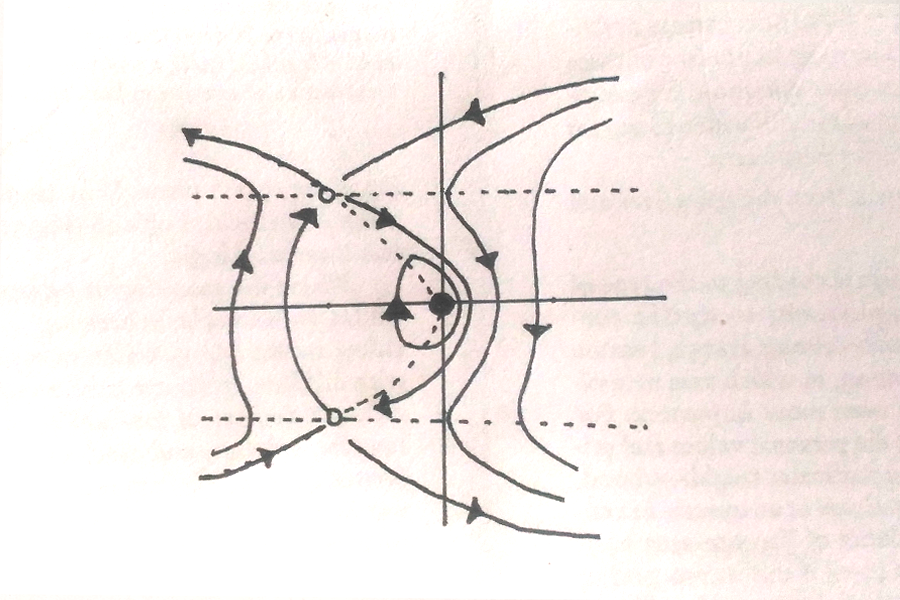
\includegraphics[width=\textwidth]{img/6-6-6e.png}
	\end{figure}
	
	\subsection*{6.6.11}
	\textbf{A.} For $t\to-t,\theta\to-\theta$: $\dot{\phi}$ is odd in $\theta$ since $\sin(-\theta) = -\sin(\theta)$ and $\dot{\theta}$ is even in $\theta$ since $\cos(-\theta)=\cos(\theta)$. Then it is reversible.
	For $t\to-t,\phi\to-\phi$: $\dot{\theta}$ is odd in $\phi$ since $\cot(-\theta)=-\cot(\theta)$ and $\dot{\phi}$ is even in $\phi$ since $\cos^2-\phi = \cos^2\phi$ and $\sin^2-\phi = \sin^2\phi$. Therefore the system is truly reversible.
	
	\textbf{B.} On Mercator projections, the phase portraits with varying A are given below.
	
	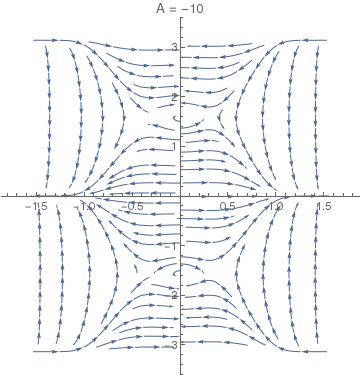
\includegraphics[width=.45\textwidth]{6611a.png}
	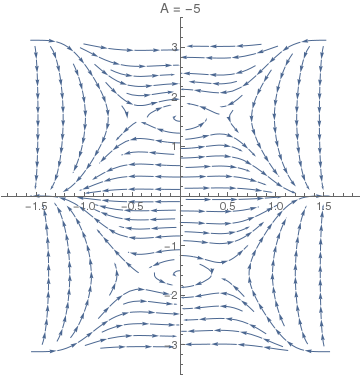
\includegraphics[width=.45\textwidth]{6611b.png}
	
	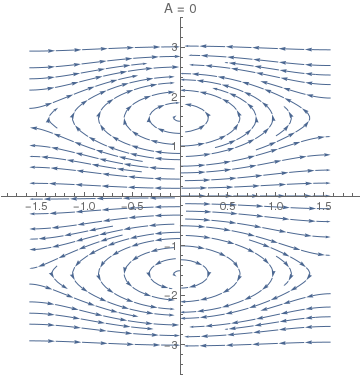
\includegraphics[width=.45\textwidth]{6611c.png}
	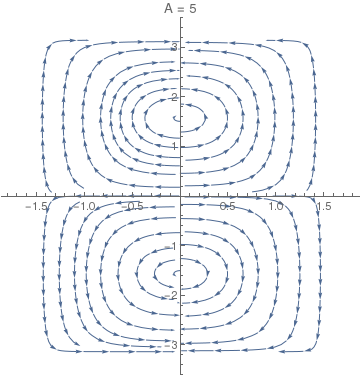
\includegraphics[width=.45\textwidth]{6611d.png}
	
	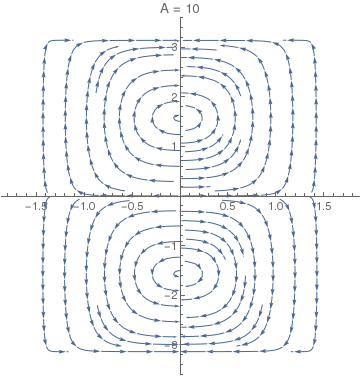
\includegraphics[width=.45\textwidth]{6611e.png}
	
	Chosen trajectories with different initial conditions on a sphere with varying A are also given below.
	
	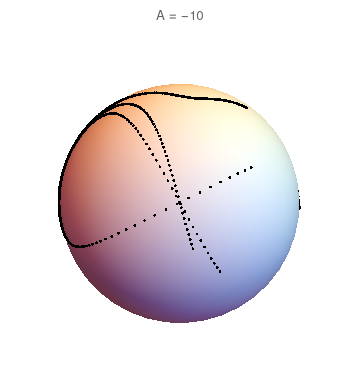
\includegraphics[width=.45\textwidth]{6611f.png}
	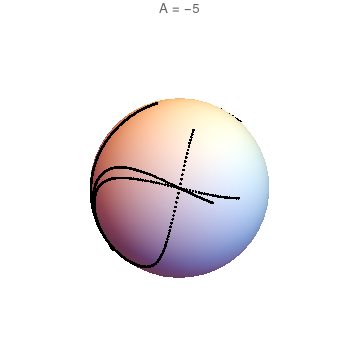
\includegraphics[width=.45\textwidth]{6611g.png}
	
	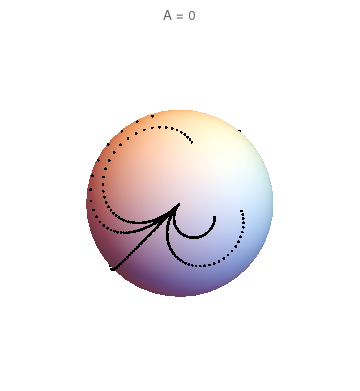
\includegraphics[width=.45\textwidth]{6611h.png}
	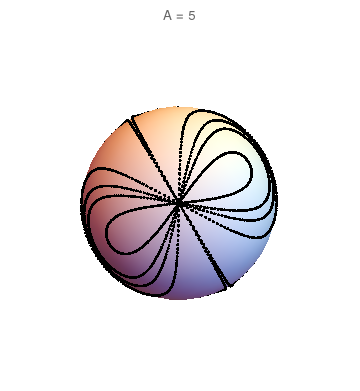
\includegraphics[width=.45\textwidth]{6611i.png}
	
	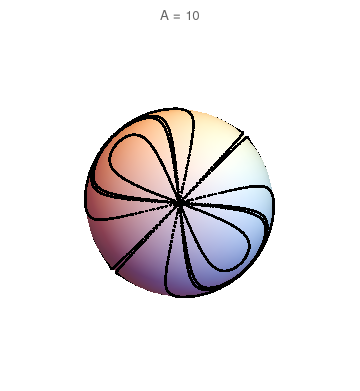
\includegraphics[width=.45\textwidth]{6611j.png}
	
	\textbf{C.} The quantities $\phi(t)$ and $\theta(t)$ represent the orientation of an object under shear flow relative to $\phi=0$ and $\theta=0$. As $t \to \infty$, the object orients to a fixed position depending on $A$ and the initial orientation. When $A>0$, there is only one possible stable orientation in $\phi$. When $A\leq0$, there are two possible stable orientations in $\phi$.
	
	\subsection*{6.7.1}
	Consider the equation for the damped pendulum, $\ddot{\theta} + b\dot{\theta} + \sin \theta = 0$, for b > 0. Linearizing this, we get $x = \dot{\theta}$ and $\dot{x} = -bx - \sin \theta$.  The Jacobian is then given by $A = \begin{bmatrix}
	-b & -\cos \theta \\
	1 & 0
	\end{bmatrix}$. \\
	Taking $b = 1$, the fixed points are then (0,0) and ($\pm \pi$, 0). \begin{align*}
	A(0,0) &= \begin{bmatrix}
	-1 & -1 \\
	1 & 0
	\end{bmatrix}  &\Delta &= 1 &\tau &= -1 \\
	A(\pm \pi,0) &= \begin{bmatrix}
	-1 & 1 \\
	1 & 0
	\end{bmatrix}  &\Delta &= 1 &\tau &= -1
	\end{align*}
	From $\Delta$ and $\tau$, (0,0) is a stable spiral while ($\pm \pi$,0) are saddles. 
	The phase portrait for b=1 is given below.\\
	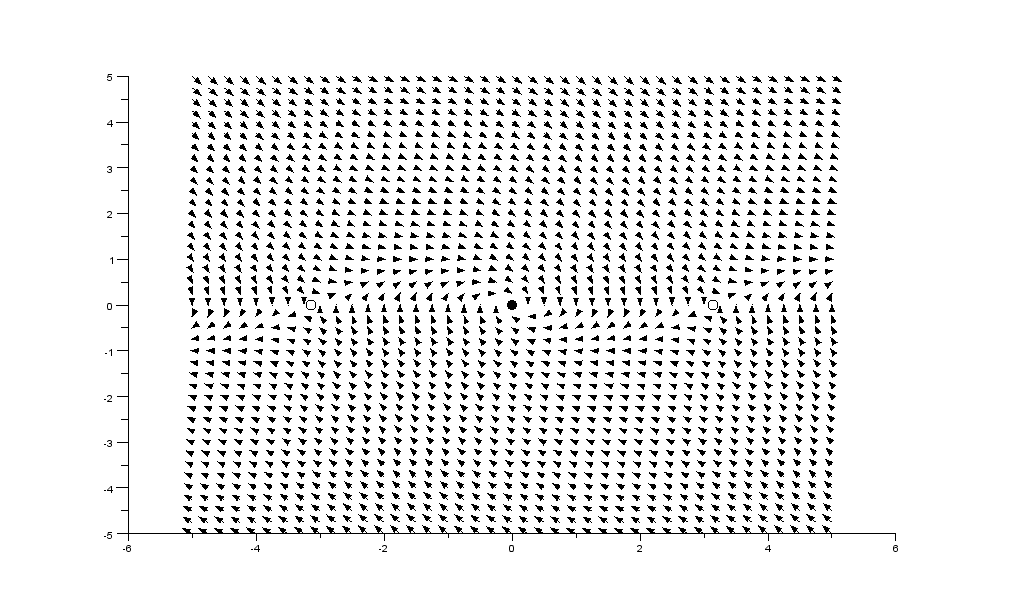
\includegraphics[width=\textwidth]{671.png}
	
	\subsection*{6.7.3}
	$\ddot \theta + (1 + a cos \theta)\dot \theta + sin\theta = 0$\\
	$\ddot \theta = -sin \theta - (1 + acos \theta)\dot \theta$\\
	
	let $\dot \theta = v$, and $\dot v = -sin \theta - (1 + acos \theta)v$. The Jacobian matrix would be
	
	\begin{equation*}
	\begin{bmatrix}
	0 & 1 \\
	-cos \theta - av sin \theta & -1 - a cos \theta
	\end{bmatrix}
	\end{equation*}
	
	\begin{align*}
	at (\pi,0): &
	\begin{bmatrix}
	0 & 1 \\
	1 & -1+a
	\end{bmatrix}
	& \tau = -1+a, \Delta = -1
	\end{align*}
	
	At $(\pi, 0)$ the equilibrium point is a saddle point since $\Delta < 0$.
	
	\begin{align*}
	at (0,0): &
	\begin{bmatrix}
	0 & 1 \\
	-1 & -1-a
	\end{bmatrix}
	& \tau = -1-a, \Delta = 1
	\end{align*}
	
	At $(0,0)$, the equilibrium point is a stable node when $a > 1$, a degenerate node when $a = 1$ and a stable spiral when $0 < a < 1$.
	
	Furthermore, the system is both not conservative and not reversible. The phase portrait of the system is shown below.
	
	\begin{figure}[H]
		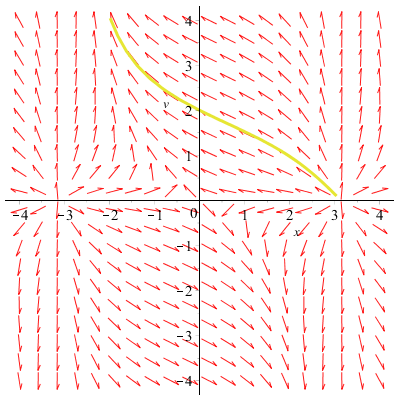
\includegraphics[width=\textwidth]{img/6-7-3.png}
	\end{figure}
	
	\subsection*{6.8.4}
	The arrow points to direction of 0 radians, then immediately to $\pi$ radians, then back to 0 radians. Therefore the index is +1.
	
	\subsection*{6.8.12}
	Consider $\dot{x} = a + x^2$ , $\dot{y} = -y$ , where $a$ is a parameter.\\
	\textbf{A.} The fixed points are $(\pm \sqrt{-a}, 0)$. The Jacobian is given by $\begin{bmatrix}
	2x & 0 \\
	0 & -1
	\end{bmatrix}.$ \\
	If $a$=0, there is a line of non-isolated fixed points. \\
	If $a < 0$, $\Delta(\sqrt{-a},0) \leq 0$, so it is a saddle point. On the other hand, $\Delta(-\sqrt{-a},0) \geq 0$, and since the eigenvalues $-2sqrt{-a}$ and -1 are real, this fixed point is a stable node. \\
	\textbf{B.} We invoke Theorem 6.8.2: any closed orbit in the phase plane must enclose fixed points whose indices sum to +1. As $a$ varies, we draw close curves that encloses all fixed points. The sum of indices of fixed points will always be conserved.
	\textbf{C.} Let $\dot{x} = f(x,a)$ where $x \in \mathbb{R^2}$ and $a$ is a parameter. Then the sum of the indices is conserved through bifurcations.\\
	Proof: Let $C$ be a closed curve enclosing all the fixed points. Then $I_C = I_1 + I_2 + ...$ where each $I_n$ is the index of a fixed point inside $C$. Now as $a$ varies, $C$ can be continuously deformed to include fixed points involved in the bifurcation. While $C$ is continuously deformed $I_C$ also varies continuously. However, $I_C$ is an integer-valued function, so it must be constant.
	
\end{document}